\documentclass[../main.tex]{subfiles}
\graphicspath{{\subfix{../../images/}}}
\begin{document}

\chapter{Basic Results}\label{chap:basic_results}

\begin{quote}
    \emph{Perception is not something that happens to us, or in us, \lbrack\ldots\rbrack It is something we do.}\\ 
    \raggedleft{--- Alva Noë, Perception in Action}
\end{quote}

\begin{quote}
    \emph{To view skilled performance as being the product of underlying component processes is to see a learning curve as a macrocosm of many individual learning experiences. Performance at one point in time reflects what has been learned at some previous time that is able to impact on performance at the moment. Thus, although a learning curve may be viewed as reflecting an incremental improvement process that leads to a smooth transition from novice to expert performance, it is actually a summary of the operation of a vast number of component processes, each with their own improvement functions, and each with varying histories of application with or without success.}\\
    \raggedleft{--- Speelman \& Kirsner, Beyond the Learning Curve}
\end{quote}

\begin{quote}
    \emph{Because some tasks require that certain components be mastered before other components can be performed or even attempted, there is likely to be a typical developmental sequence in acquiring certain skills. Furthermore, if substantial work is required for component processes to reach a level of mastery before higher level tasks can be attempted, then there is likely to be some period of consolidation in the acquisition of the higher level skill. That is, there will be periods in which there appears to be little progress being made in performance of the task. Closer scrutiny, however, may reveal that performance is improving, but only on lower level components of the task. According to this view of skill acquisition, then, the processes that underlie plateaus in learning curves may also underlie the stages that are characteristic of cognitive development}\\
    \raggedleft{Piaget, 1953}
\end{quote}

\begin{quote}
    \emph{Learning is not like a coin, which remains physically whole even through the most infamous transactions; it is, rather, like a very handsome dress, which is worn out through use and ostentation.}
    \raggedleft{--- Umberto Eco, The Name of the Rose}
\end{quote}


\cleardoublepage%








%%%%%% PERFORMANCE OVER BLOCKS

\section{Task Performance}

What results that tell us the tasks are working as we intended? What confirms that our experimental design is sound measured against our aims?
 
- What separates learners into high and low performers? What predicts differences in performance?
- We want to look at intersubject variability– do people use similar “strategies”?
- Do subjects end up using statistically similar solutions?
- Explain learning from a statistical point of view– what is actually being learned? Is there a general learning principle across subjects?


we see an interaction between learning systems -- cortex, cerebellum, basal ganglia -- strategy / unsupervised prediction / supervised, RL / policies?
this leads to multiple learning rates, fast and slow learning, discontinuities in learning

questions -- what information influences learning?
that is, what projection of the data best explains performance increases?
is this projection / this information the same across participants?

skill learning will lead to hierarchy, and different levels of the hierarchy may be learned at different times by different means/systems

what is the mostly likely deconvolution of the learning curve?

what do our learning curves look like? plateaus? discontinuities?
can we measure performance within trial? (movement towards target at each time step?)

what you're learning is dimensions of goal-relevance... as these dimensions are learned, we see changes in variability and in performance








\begin{figure}[H]
    \centering
    \includegraphics[width=1.0\textwidth]{basic_results/performance_over_blocks/hits_and_noholds.pdf}
    \caption[Hit counts over trials]{}\label{fig:hits_and_noholds}
\end{figure}


\begin{figure}[H]
    \centering
    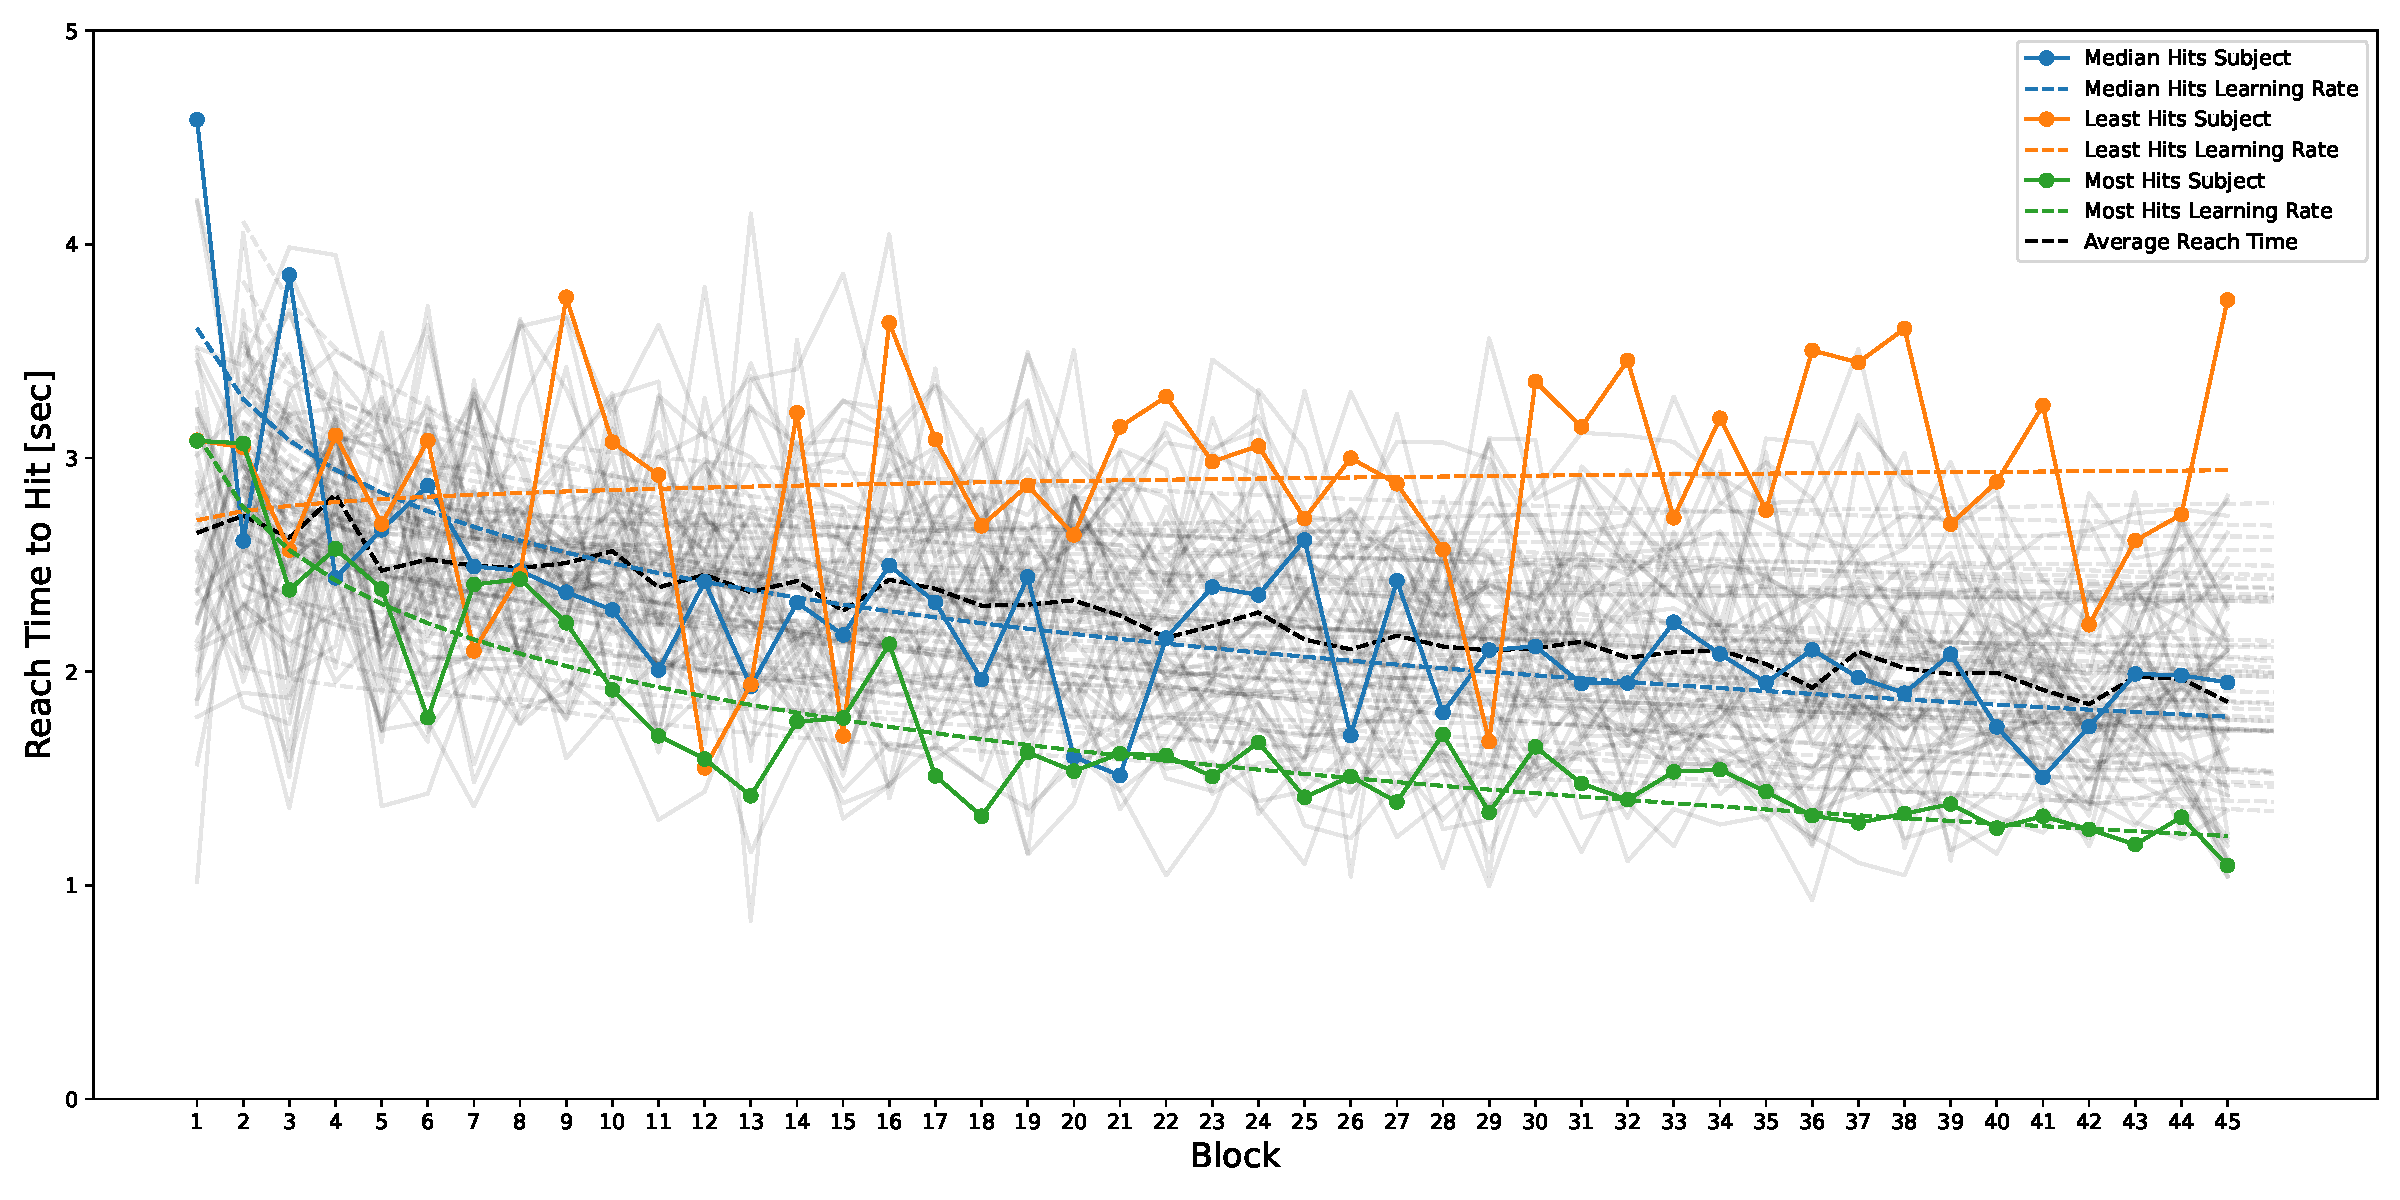
\includegraphics[width=1.0\textwidth]{basic_results/performance_over_blocks/reach_times_over_blocks.pdf}
    \caption[Reach time over trials]{}\label{fig:reach_times_over_blocks}
\end{figure}


\begin{figure}[H]
    \centering
    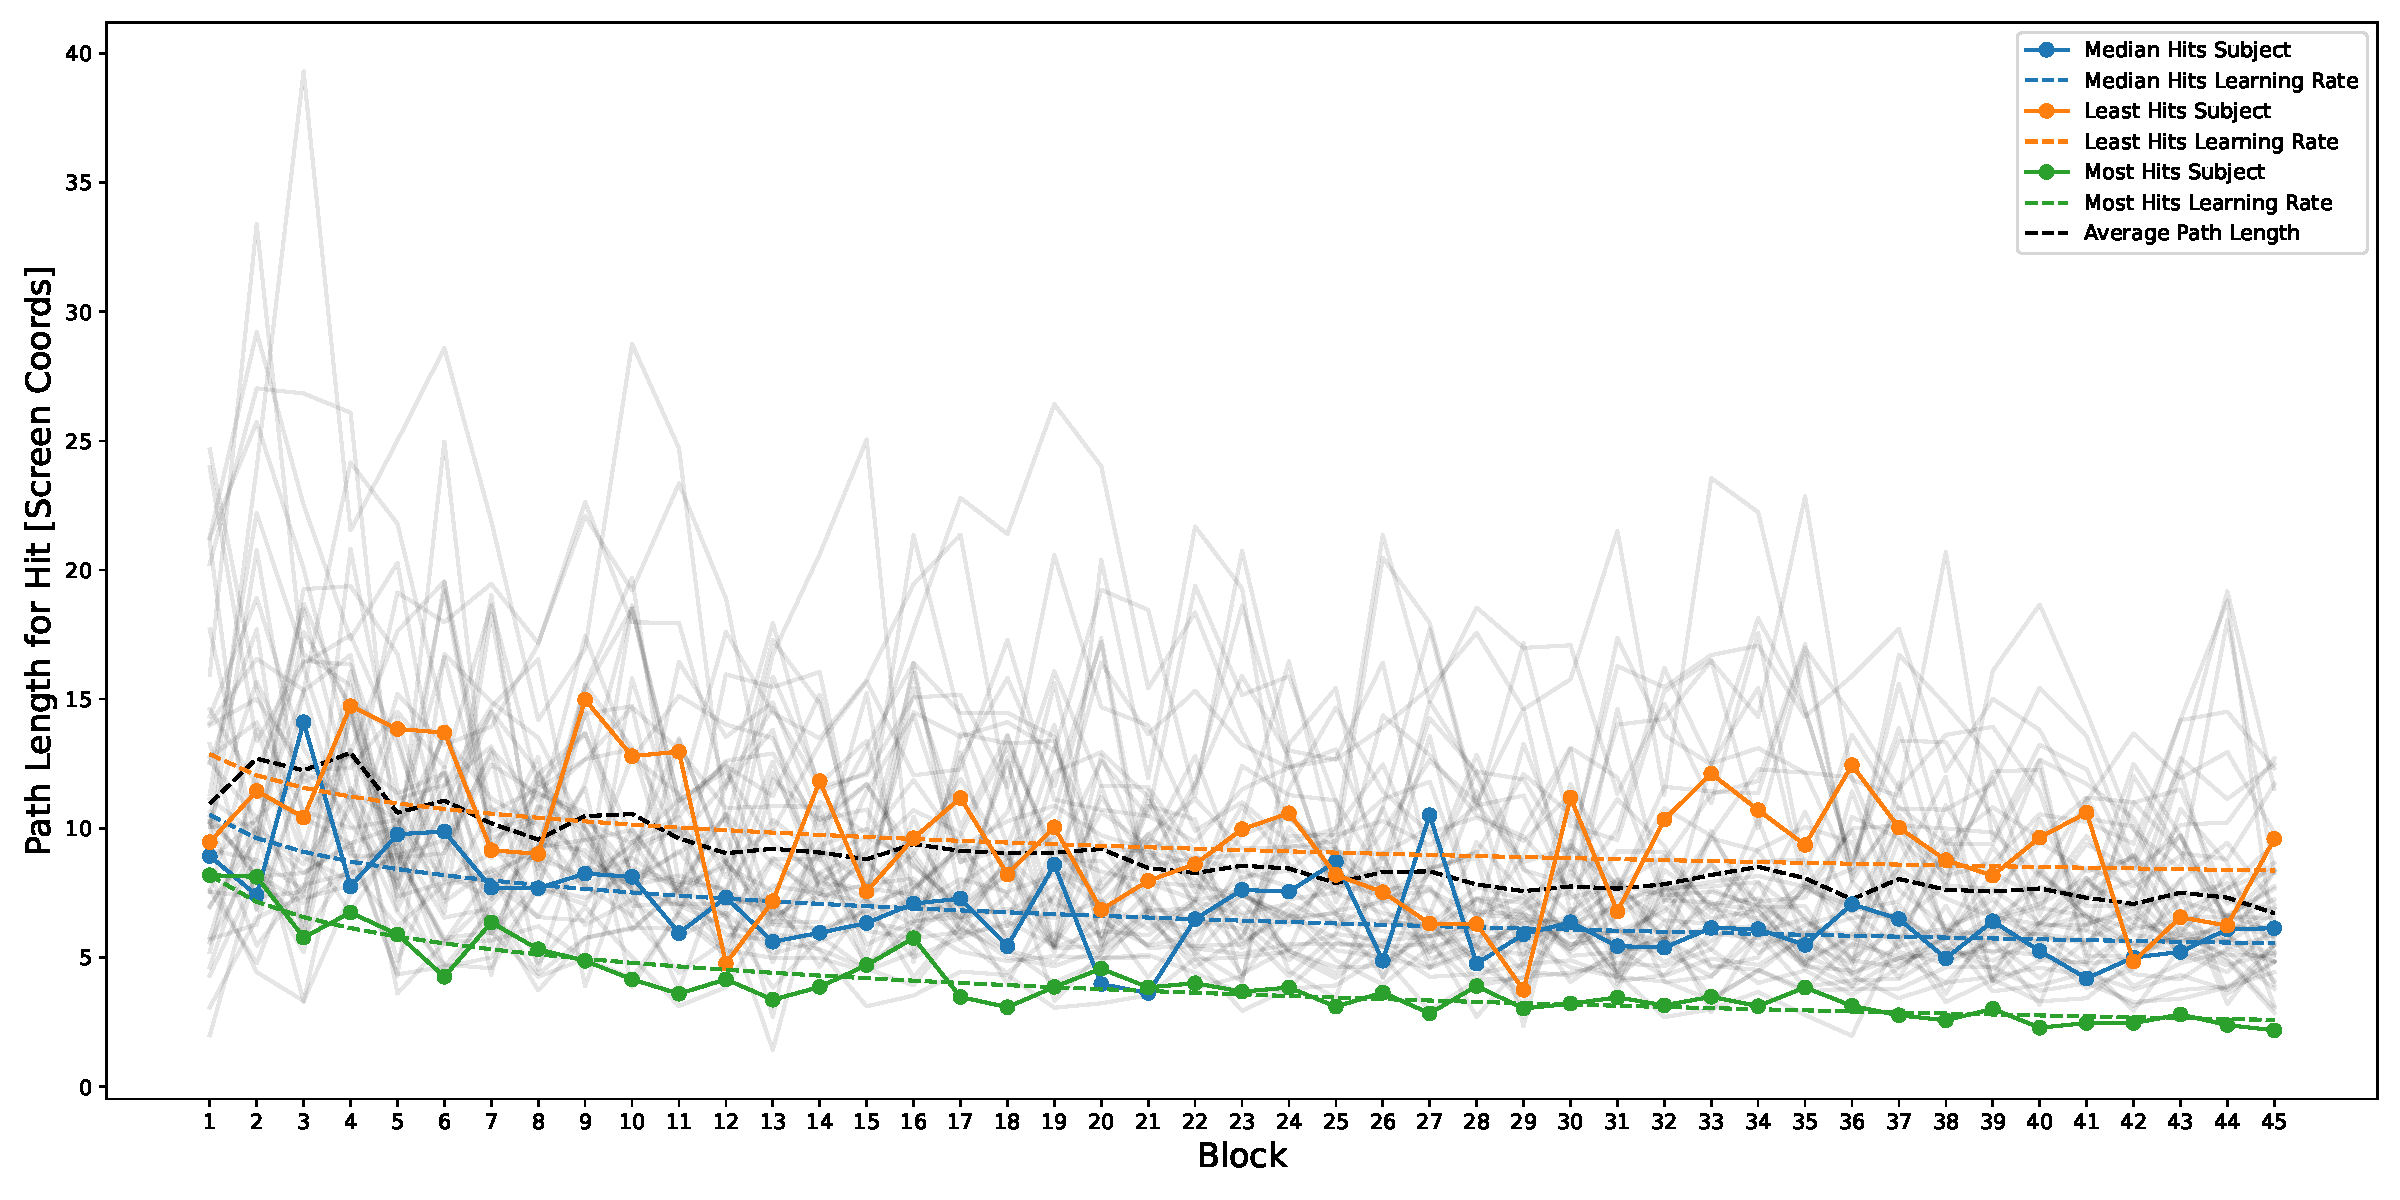
\includegraphics[width=1.0\textwidth]{basic_results/performance_over_blocks/path_length_over_blocks.pdf}
    \caption[Trajectory length over trials]{return np.sum (np.sqrt (np.sum (np.diff (a, axis=0)**2,axis=1)))}\label{fig:path_length_over_blocks}
\end{figure}


\begin{figure}[H]
    \centering
    \includegraphics[width=1.0\textwidth]{basic_results/performance_over_blocks/path_segments_over_blocks.pdf}
    \caption[Trajectory segments over trials]{This connects to the idea of freezing degrees of freedom. We expect to see degrees of freedom in the task space, quantified by segments, to decrease over trials.}\label{fig:path_segments_over_blocks}
\end{figure}


\begin{figure}[H]
    \centering
    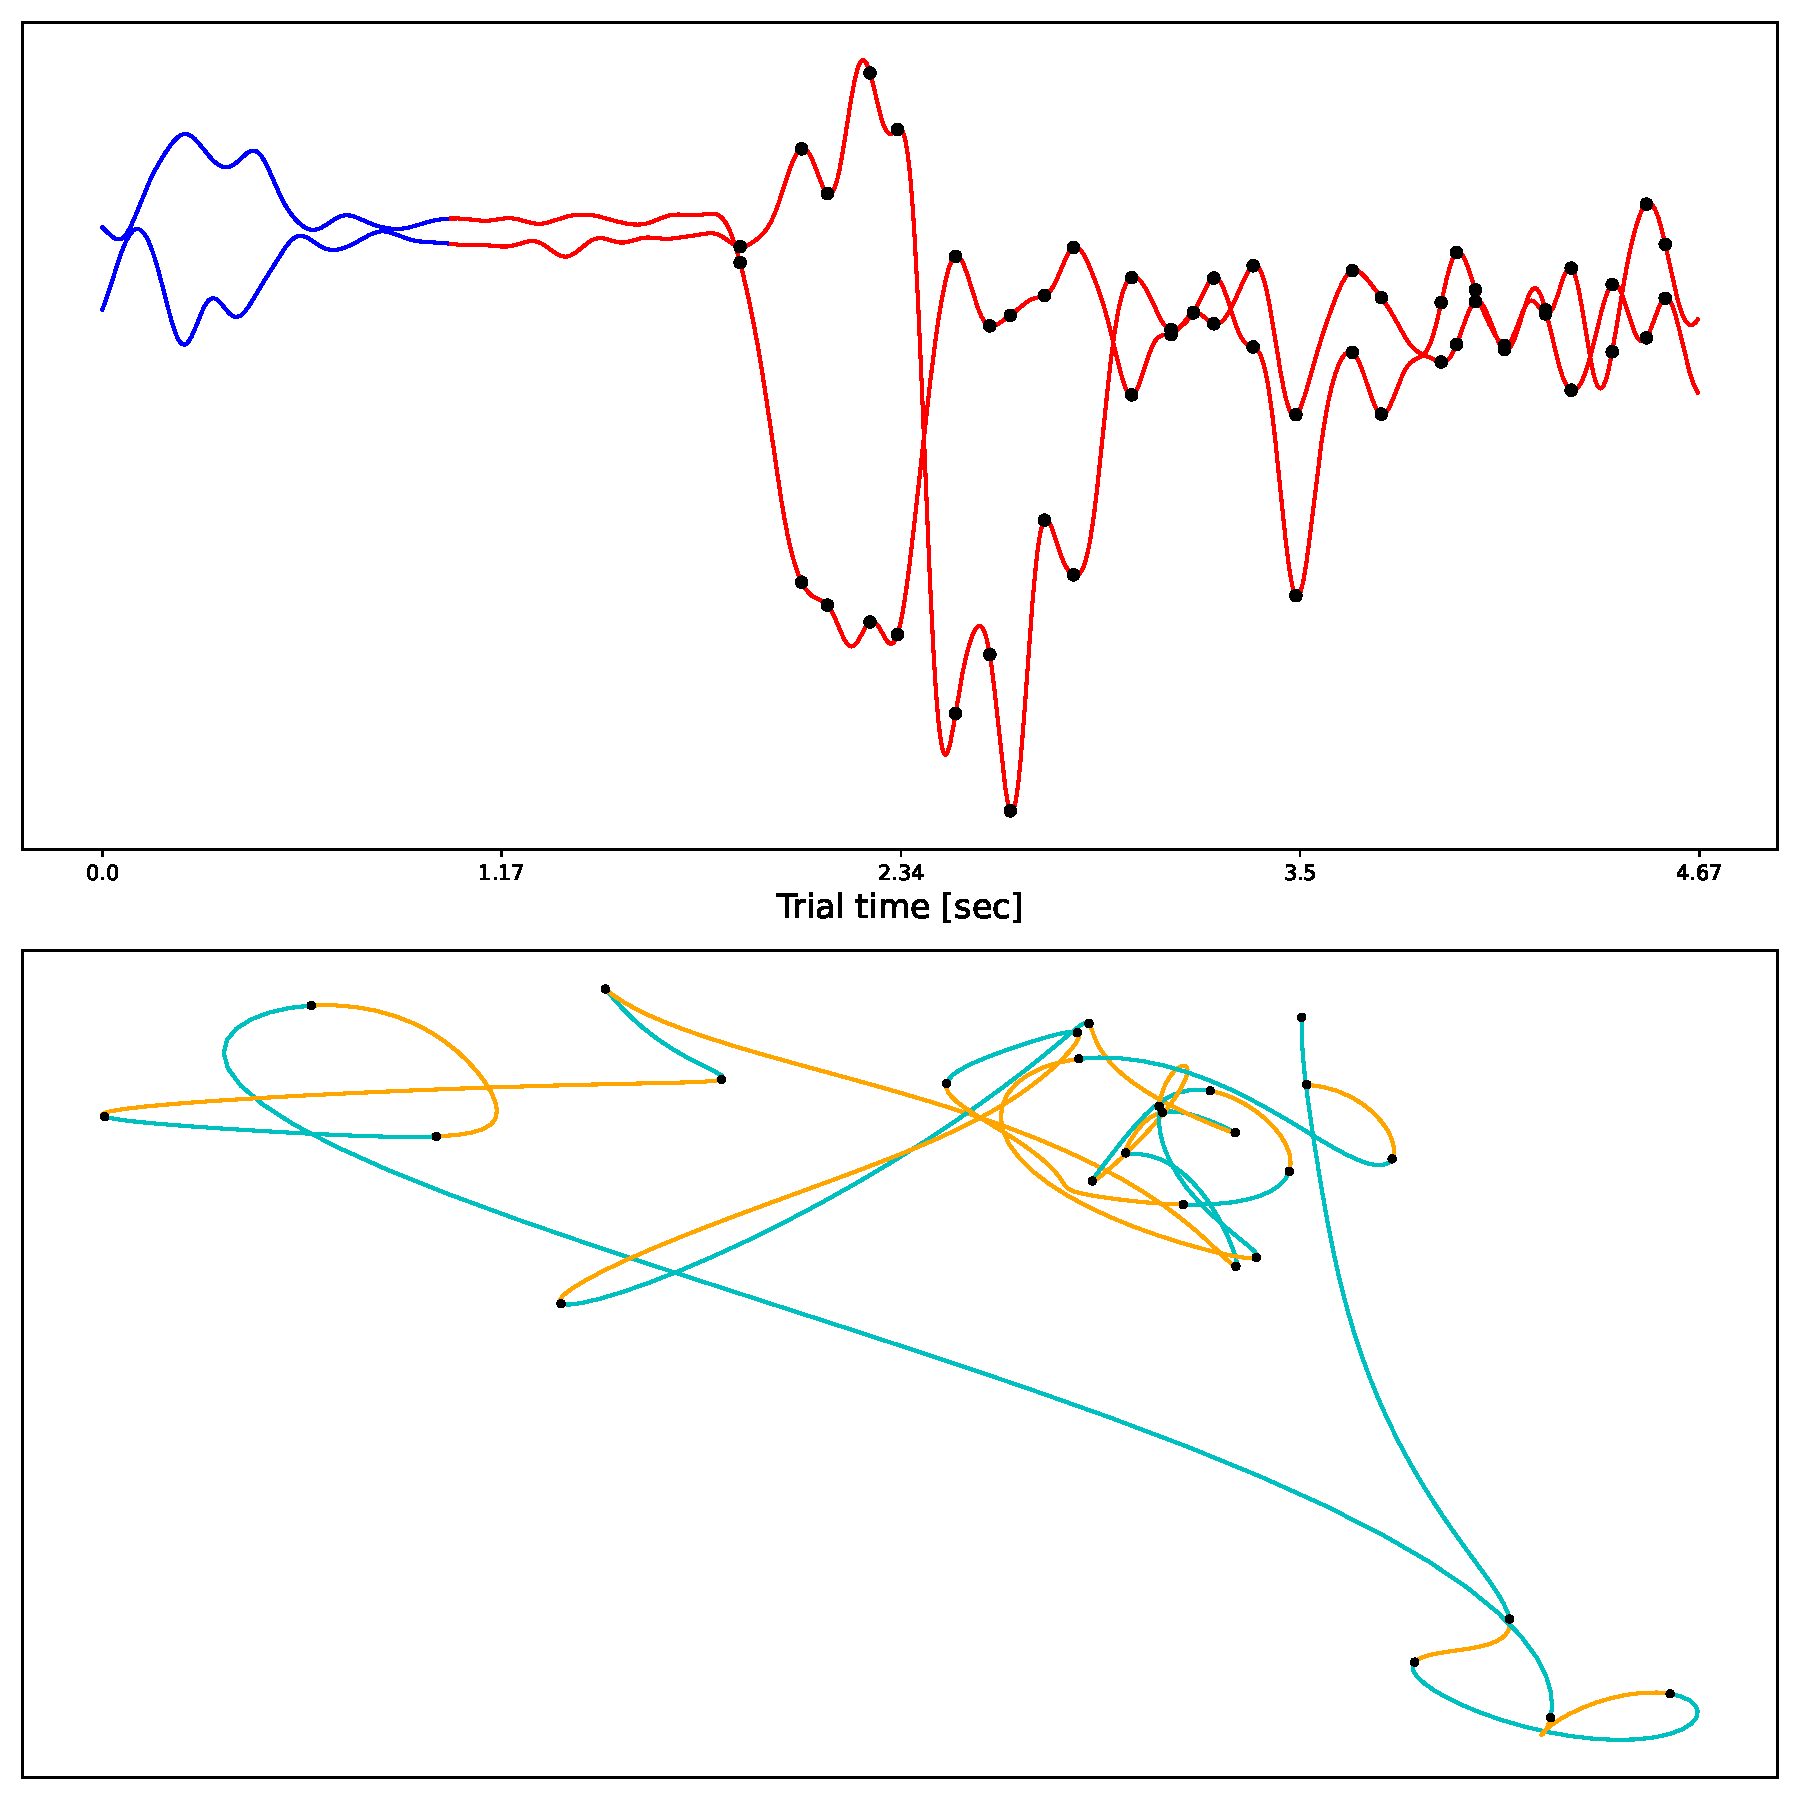
\includegraphics[width=1.0\textwidth]{basic_results/performance_over_blocks/example_path_segments.pdf}
    \caption[Trajectory segment definition]{zero crossings are diff (sign (diff (x))), then filter crossings that are within a time interval and above a minimum velocity as a percentage of the max}\label{fig:segments}
\end{figure}


\begin{figure}[H]
    \centering
    \includegraphics[width=0.8\textwidth]{basic_results/performance_over_blocks/hit_fraction_vs_reward.pdf}
    \caption[Hits versus reward]{Fractions of trial outcome types for each block of the center-hold, reach-out task. Hit fraction increases on each trial, suggesting the beginnings of task learning. Hold timeout failure increases over trials as well, perhaps suggesting increased baseline excitation of muscles during the hold period. Part of learning to activate certain muscle modes is learning to inhibit others.}\label{fig:hit_fraction_vs_reward}
\end{figure}

Reward is defined over $K$ trials and samples or timepoints $T$ as:

\begin{align}
    r = \frac{1}{KT}\sum_k^K\sum_t^T{|| \vec{g_k} - \vec{x}_{t,k} ||^2}.
    \label{eq:reward}
\end{align}

\cref{eq:reward}


\begin{figure}[H]
    \centering
    \includegraphics[width=1.0\textwidth]{basic_results/performance_over_blocks/mean_rewards_vs_learning_rate.pdf}
    \caption[Reward versus learning rate]{No correlation!}\label{fig:mean_rewards_vs_learning_rate}
\end{figure}



\begin{figure}
    \centering
    \begin{minipage}{0.49\textwidth}
        \includegraphics[width=0.9\textwidth]{basic_results/trial_reward/reward_histogram.pdf}
        \subcaption{}
    \end{minipage}
    \begin{minipage}{0.49\textwidth}
        \includegraphics[width=0.9\textwidth]{basic_results/trial_reward/hit_fraction_histogram.pdf}
      \subcaption{}
    \end{minipage}
    \caption[Hit and reward histograms]{Hits and rewards}\label{fig:reward_histograms}
\end{figure}


\begin{figure}[H]
    \centering
    \includegraphics[width=1.0\textwidth]{basic_results/pca_dimensionality/PCA_variance.pdf}
    \caption[Explained variance over tasks]{No correlation!}\label[figure]{pca_variance}
\end{figure}

\begin{table}
    \begin{center}
        \caption[Statistics of peformance regression]{}\label{}
        \begin{tabular}{l | c}
            \hline
            $p$(Hit Learning Rate, Reward) & 0.177 \\
            $p$(Reach time Learning Rate, Reward) & 0.215 \\
            $p$(Path length Learning Rate, Reward) & 0.786 \\
            $p$(Segment Learning Rate, Reward) & 0.072 \\
            Adjusted R-squared & 0.058 \\
            Prob (F-statistic) & 0.170
        \end{tabular}
    \end{center}
\end{table}

% \clearpage
% \begin{table}[H]
% \begin{center}
%     \caption{$p$-values for \Cref{pca_variance}}\label{table:pvalues}
%     \begin{tabular}{l | c}
%         Variable & $p$ Value \\
%         \hline
%         \cellcolor{red!25} Calibration --- Movement & \cellcolor{red!25} 9.644e-09 \\
%         \cellcolor{red!25} Trial Block 1 --- Movement & \cellcolor{red!25} 9.348e-05 \\
%         Trial Block 1 --- Calibration & 5.684e-01 \\
%         \cellcolor{red!25} Trial Block 2 --- Movement & \cellcolor{red!25} 5.591e-05 \\
%         Trial Block 2 --- Calibration & 6.444e-01 \\
%         Trial Block 2 --- Trial Block 1 & 1.000e+00 \\
%         \cellcolor{red!25} Trial Block 3 --- Movement & \cellcolor{red!25} 1.255e-02 \\
%         \cellcolor{red!25} Trial Block 3 --- Calibration & \cellcolor{red!25} 4.340e-02 \\
%         Trial Block 3 --- Trial Block 1 & 8.755e-01 \\
%         Trial Block 3 --- Trial Block 2 & 8.230e-01 \\
%         \cellcolor{red!25} Trial Block 4 --- Movement & \cellcolor{red!25} 2.040e-02 \\
%         \cellcolor{red!25} Trial Block 4 --- Calibration & \cellcolor{red!25} 2.786e-02 \\
%         Trial Block 4 --- Trial Block 1 & 8.039e-01 \\
%         Trial Block 4 --- Trial Block 2 & 7.394e-01 \\
%         Trial Block 4 --- Trial Block 3 & 1.000e+00 \\
%         \cellcolor{red!25} Trial Block 5 --- Movement & \cellcolor{red!25} 2.762e-02 \\
%         \cellcolor{red!25} Trial Block 5 --- Calibration & \cellcolor{red!25} 2.058e-02 \\
%         Trial Block 5 --- Trial Block 1 & 7.487e-01 \\
%         Trial Block 5 --- Trial Block 2 & 6.783e-01 \\
%         Trial Block 5 --- Trial Block 3 & 1.000e+00 \\
%         Trial Block 5 --- Trial Block 4 & 1.000e+00 \\
%         \end{tabular}
% \end{center}
% \end{table}


\begin{figure}[H]
    \centering
    \includegraphics[width=1.0\textwidth]{basic_results/pca_dimensionality/pca_pvalues.pdf}
    \caption[Explained variance Tukey test]{$p$-values for Tukey's honestly significant difference test for pairwise means of a group of samples. Here we compare the explained variance of the top two singular values for the movement, calibration, and 5 blocks of task trials over subjects.}\label{fig:pca_pvalues}
\end{figure}

\Cref{fig:pca_pvalues}

% The observations being tested are independent within and among the groups.
% The groups associated with each mean in the test are normally distributed.
% There is equal within-group variance across the groups associated with each mean in the test (homogeneity of variance).



\begin{figure}[H]
    \centering
    \begin{minipage}{0.49\textwidth}
        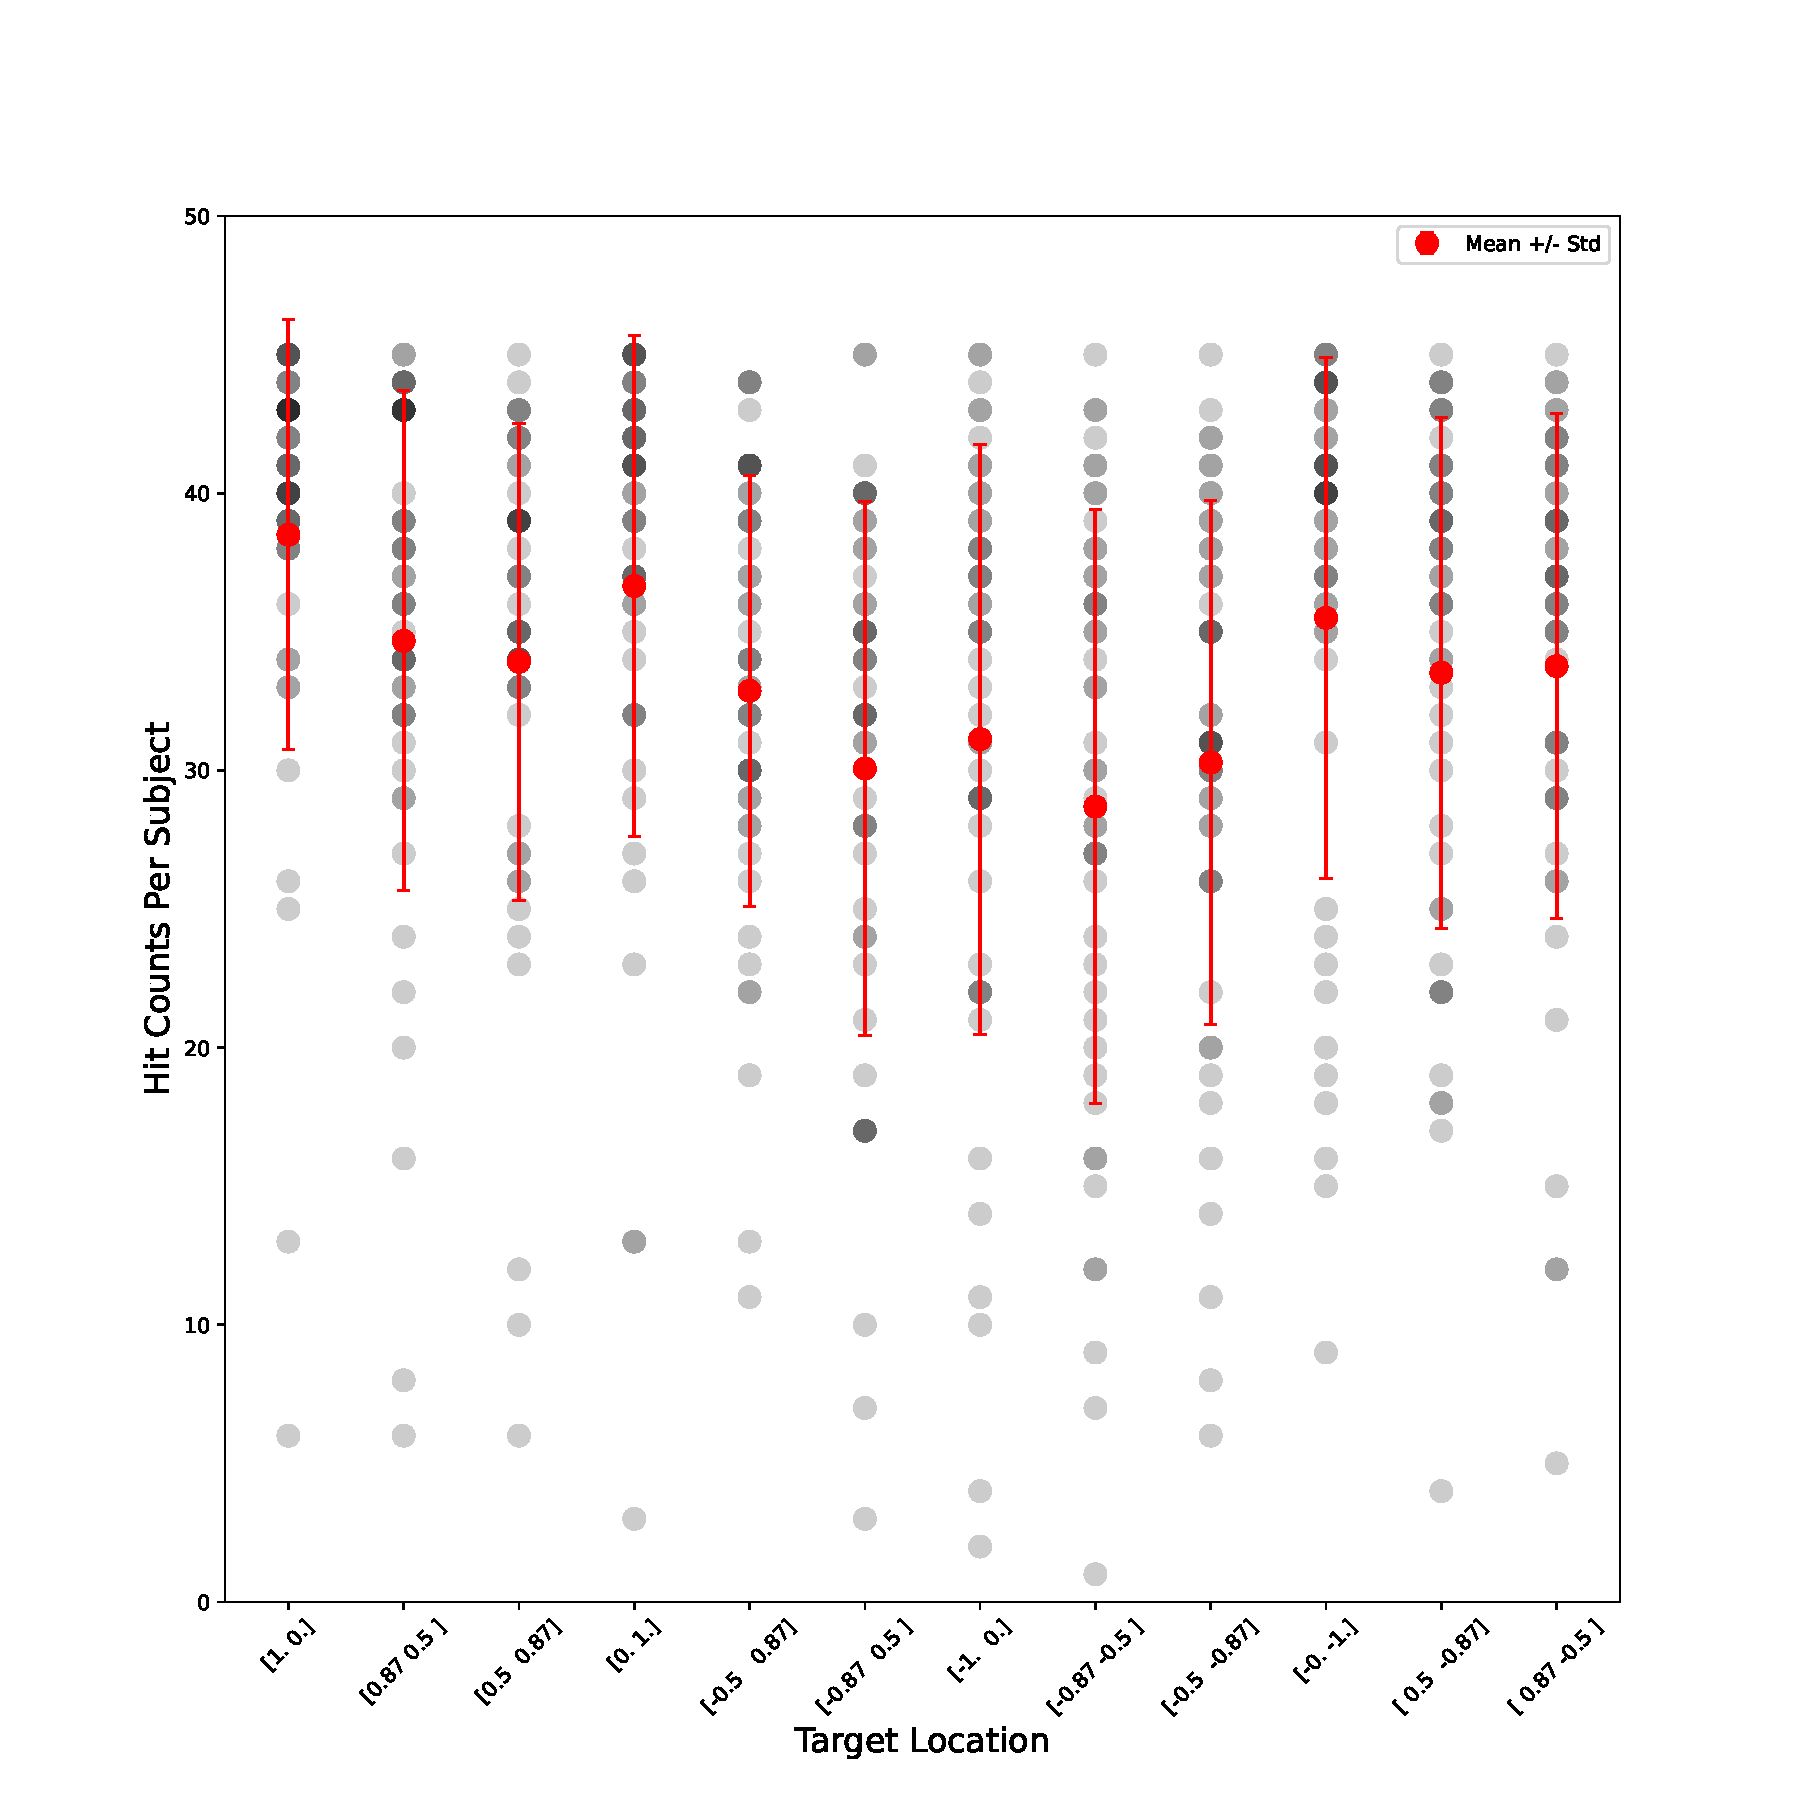
\includegraphics[width=0.95\textwidth]{basic_results/decoder_vs_performance/hits_over_targets.pdf}
        \subcaption{}
    \end{minipage}
    \begin{minipage}{0.49\textwidth}
        \includegraphics[width=0.85\textwidth]{basic_results/decoder_vs_performance/target_means.pdf}
      \subcaption{}
    \end{minipage}
    \caption[Hits over targets]{Hits over targets}\label{fig:hits_over_targets}
\end{figure}


\begin{figure}[H]
    \centering
    \includegraphics[width=0.8\textwidth]{basic_results/decoder_vs_performance/target_hit_pvalues.pdf}
    \caption[Target hit Tukey test]{??}\label{fig:target_hit_pvalues}
\end{figure}

\cref{fig:target_hit_pvalues}
\cref{fig:target_hit_pvalues}


% Table showing p-values for target subject mean hit fraction differences:
% 
% \begin{table}[H]
% \begin{center}
%     \caption{}\label{table:}
%     \begin{tabular}{ c | c }
%         Target Pair & $p$-value \\
%         \hline
%         1, 6  & 1.085e-03 \\ 
%         1, 7  & 9.567e-03 \\ 
%         1, 8  & 4.629e-05 \\ 
%         1, 9  & 1.830e-03 \\ 
%         4, 6  & 4.040e-02 \\ 
%         4, 8  & 3.251e-03 \\ 
%         8, 10  & 2.783e-02 \\ 
%     \end{tabular}
% \end{center}
% \end{table}

\begin{figure}[H]
    \centering
    \includegraphics[height=0.9\textheight]{basic_results/mean_trajectories/mean_trajectories.pdf}
    \caption[Mean trajectories]{??}\label{fig:mean_trajectories}
\end{figure}

\begin{figure}[H]
    \centering
    \includegraphics[height=0.9\textheight]{basic_results/trajectory_variance/rotated_trajectories.pdf}
    \caption[Rotating trajectories]{??}\label{fig:rotated_trajectories}
\end{figure}


\begin{figure}[H]
    \centering
    \includegraphics[height=0.9\textheight]{basic_results/trajectory_variance/trajectory_variance_over_blocks.pdf}
    \caption[Trajectory variance over blocks]{Plotting the log as variance tends to decrease exponentially}\label{fig:trajectory_variance}
\end{figure}


\begin{figure}[H]
    \centering
    \begin{minipage}{0.49\textwidth}
        \includegraphics[width=0.95\textwidth]{basic_results/trajectory_variance/trajectory_r_squared_fit.pdf}
        \subcaption{}
    \end{minipage}
    \begin{minipage}{0.49\textwidth}
        \includegraphics[width=0.85\textwidth]{basic_results/trajectory_variance/trajectory_variance_slope.pdf}
      \subcaption{}
    \end{minipage}
    \caption[Trajectory variance statistics]{Hits over targets}\label{fig:trajectory_variance_fits}
\end{figure}










%%%%%% FORM RESPONSES

\section{Self-reported Subject Form Data}

\begin{figure}[H]
    \centering
    \includegraphics[width=1.0\textwidth]{basic_results/form_response/compare_subject_groups.pdf}
    \caption[Subject group comparisons]{}\label{fig:compare_subject_groups}
\end{figure}


\begin{figure}[H]
    \centering
    \includegraphics[width=1.0\textwidth]{basic_results/form_response/arm_vs_reward.pdf}
    \caption[Arm versus reward]{}\label{fig:arm_vs_reward}
\end{figure}

\begin{figure}[H]
    \centering
    \includegraphics[width=1.0\textwidth]{basic_results/form_response/days_vs_reward.pdf}
    \caption[Experiment day versus reward]{}\label{fig:days_vs_reward}
\end{figure}

\begin{figure}[H]
    \centering
    \includegraphics[width=1.0\textwidth]{basic_results/form_response/hour_of_day_vs_reward.pdf}
    \caption[Hour of day versus reward]{}\label{fig:hour_of_day_vs_reward}
\end{figure}

\begin{figure}[H]
    \centering
    \includegraphics[width=1.0\textwidth]{basic_results/form_response/sleep_vs_reward.pdf}
    \caption[Hours of sleep vs reward]{}\label{fig:sleep_vs_reward}
\end{figure}
















%%%%%% DECODER 

\section{Decoder}

\begin{figure}[H]
    \centering
    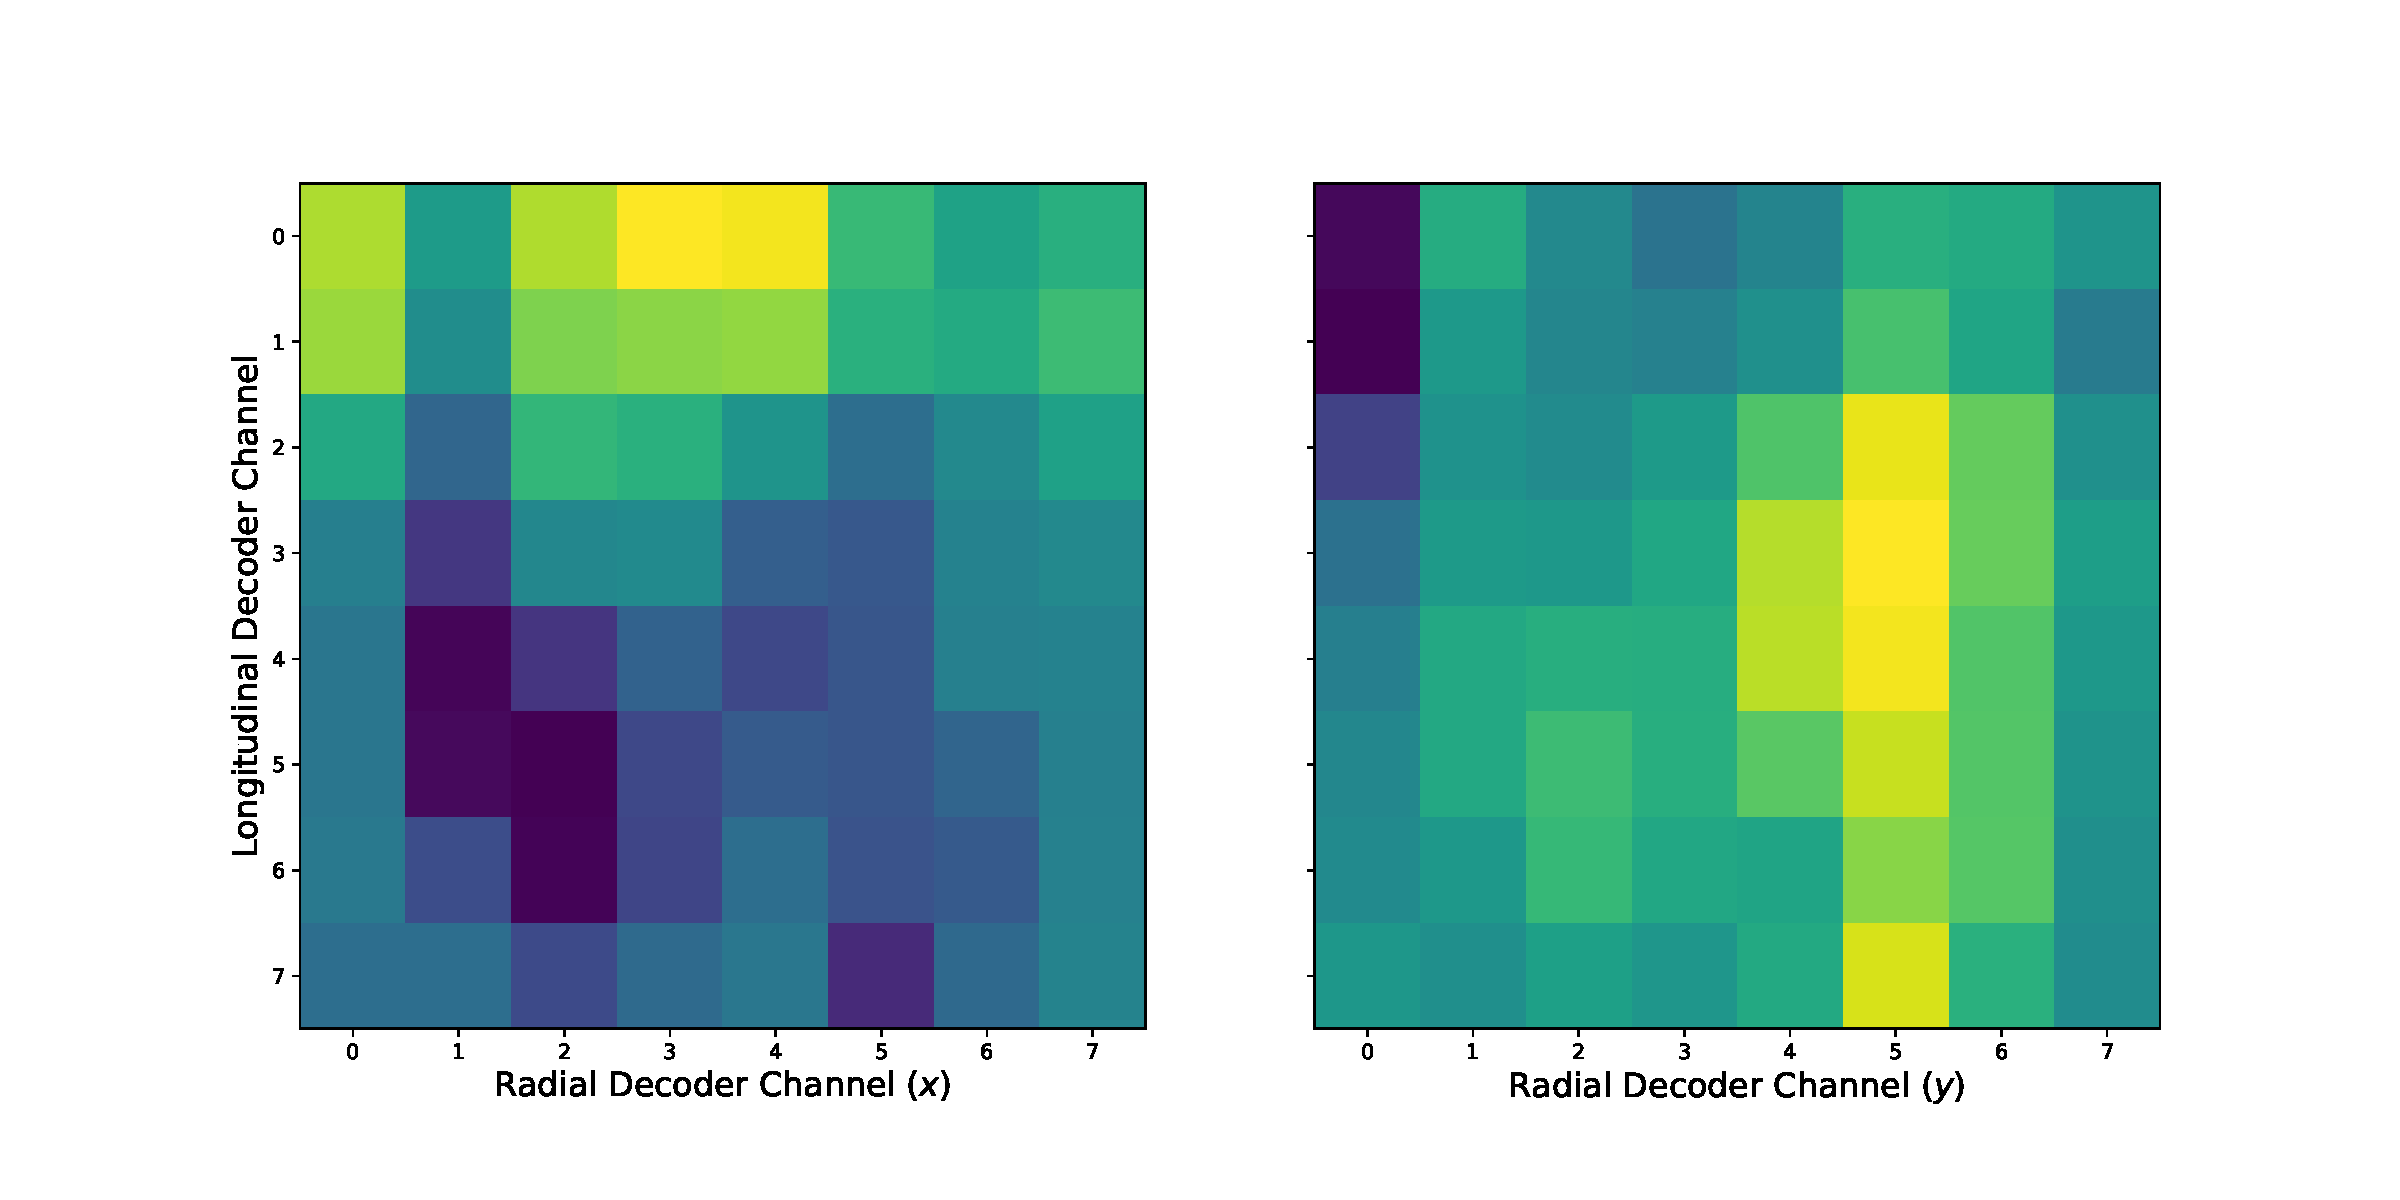
\includegraphics[width=1.0\textwidth]{basic_results/performance_over_blocks/example_decoder.pdf}
    \caption[Example subject decoder]{}\label{fig:example_decoder}
\end{figure}

\begin{figure}[H]
    \centering
    \includegraphics[height=1.0\textheight]{basic_results/decoder_vs_performance/decoder_arrows.pdf}
    \caption[Example decoder directions in 2D.]{Example decoders directions in 2D.}\label{fig:decoder_arrows}
\end{figure}

\begin{figure}[H]
    \centering
    \includegraphics[width=1.0\textwidth]{basic_results/decoder_vs_performance/decoder_normality_test.pdf}
    \caption[Decoder normality testing]{Testing the effect of the decoder on uniform data.}\label{fig:decoder_normality}
\end{figure}

\begin{figure}[H]
    \centering
    \includegraphics[width=1.0\textwidth]{basic_results/decoder_vs_performance/decoder_cosine_vs_reward.pdf}
    \caption[Decoder axis similarity versus reward]{No correlation!}\label{fig:decoder_cosine_vs_reward}
\end{figure}






%%%%%% DATA SHAPE

\section{EMG Correlations}

\begin{figure}[H]
    \centering
    \includegraphics[width=1.0\textwidth]{basic_results/pairplot/raw_pairplot.png}
    \caption[Pairplot of calibration data]{Pairplot of calibration data}\label{fig:raw_pairplot}
\end{figure}

\begin{figure}[H]
    \centering
    \includegraphics[width=1.0\textwidth]{basic_results/pairplot/log_pairplot.png}
    \caption[Pairplot of log-transformed calibration data]{Pairplot of log-transformed calibration data}\label{fig:log_pairplot}
\end{figure}


% mean_reward vs [hit_learning_rates, reach_time_learning_rates, path_length_learning_rates, segment_learning_rates]

% OLS Regression Results                            
% ==============================================================================
% Dep. Variable:                      y   R-squared:                       0.142
% Model:                            OLS   Adj. R-squared:                  0.058
% Method:                 Least Squares   F-statistic:                     1.693
% Date:                Wed, 14 Feb 2024   Prob (F-statistic):              0.170
% Time:                        10:31:57   Log-Likelihood:               -0.99915
% No. Observations:                  46   AIC:                             12.00
% Df Residuals:                      41   BIC:                             21.04
% Df Model:                           4                                         
% Covariance Type:            nonrobust                                         
% ==============================================================================
%                  coef    std err          t      P>|t|      [0.025      0.975]
% ------------------------------------------------------------------------------
% const          0.9233      0.114      8.083      0.000       0.693       1.054
% x1             0.0780      0.057      1.375      0.177      -0.037       0.193
% x2             0.7350      0.584      1.259      0.215      -0.444       1.914
% x3             0.0102      0.037      0.274      0.786      -0.065       0.085
% x4            -0.1088      0.059     -1.845      0.072      -0.228       0.010
% ==============================================================================
% Omnibus:                        4.990   Durbin-Watson:                   2.155
% Prob(Omnibus):                  0.083   Jarque-Bera (JB):                4.054
% Skew:                           0.477   Prob(JB):                        0.132
% Kurtosis:                       4.098   Cond. No.                         51.4
% ==============================================================================








%%%%%% PCA DIMENSIONALITY 







% \begin{figure}[H]
% \phantomsection\label{fig:PCA_trial_variance}
% \centering
% 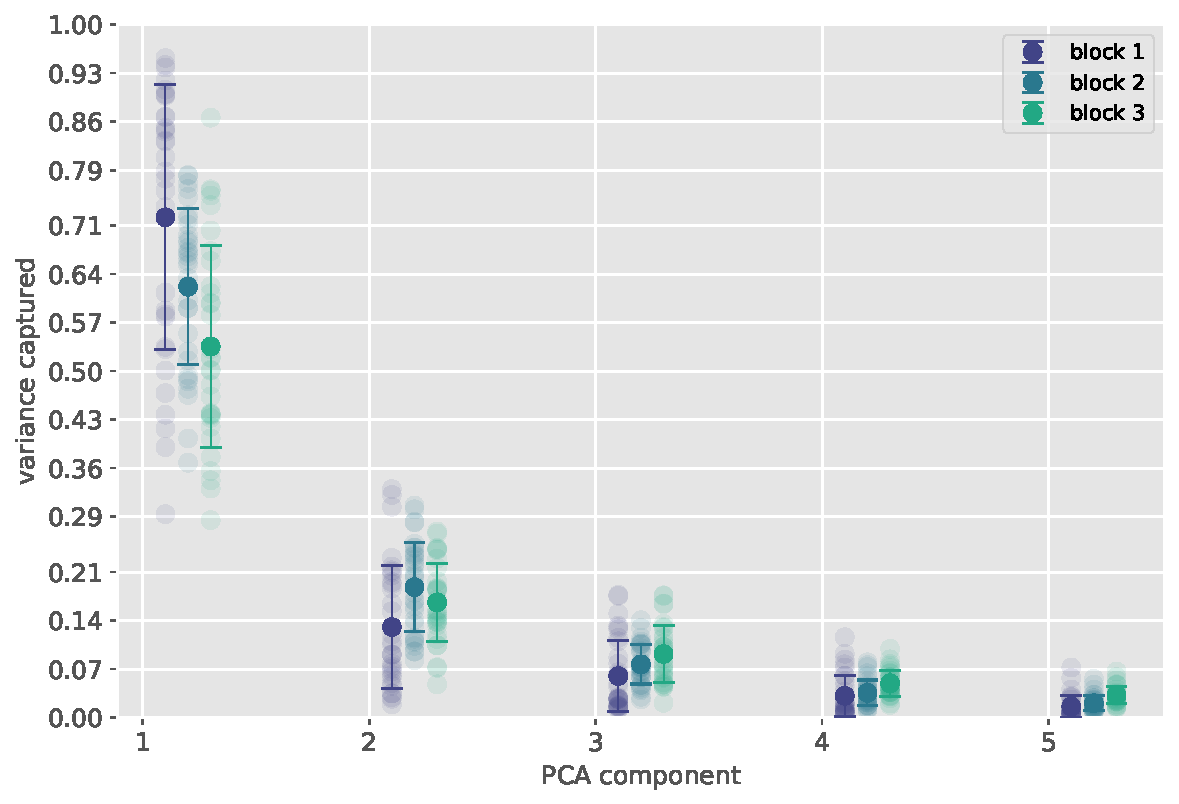
\includegraphics[width=0.2\textwidth]{images/data_analysis/center_hold/PCA_trial_variance.pdf}
% \caption{Fraction of variance captured by the top five principle components when PCA is run on the EMG time series' of individual trials of the center-hold, reach-out task. Error bars are standard deviation. Over blocks, we see a slight decrease in the mean of the top component's variance fraction, though with high variance. This may suggest greater exploration within-trial, as less variance is captured by a single component over blocks, though it could reflect more varied dynamics across trials as the subject discovers new, task-relevant activations.}\label{fig:PCA_trial_variance}
% \end{figure}

% We might model this task as the subject selecting an EMG signal $x$ which minimizes the distance between a target position $b$ and the projection of the EMG signal through the mapping $M$ as well as minimizes the norm of $x$ in order to conserve metabolic energy. This optimization can be written as a regularized least squares problem:

% \begin{align}
%   \min_x\frac{1}{2}||Mx - b||^2_2 + \frac{\lambda}{2}||x||_2^2.
% \end{align}

% This problem is known to have a unique minimum for $\lambda>0$ which is an approximation $Mx\approx b$ regardless of the shape or rank of $M$. This implies that the subject, if they are biophysically capable to do so, will learn distinct motor outputs for each target rather than reusing modes for multiple targets with different activation levels. That is the subject will, over time, learn to fractionate their muscle output to reach their goal in order to minimize effort. For instance, to reach the the target at position $(1,0)$ in Cartesian coordinates, the subject could activate a bespoke activity mode and activate a combination of two or more modes for targets at $\pm45^\circ$ from this central target. If this is the case, the model predicts that the dimensionality of the EMG signal will increase over the course of training as the subject learns to construct bespoke activity modes for each target.


% \section{Policy Complexity}

% PCA subspace dimensionality
% Entropy!


% In \Cref{fig:PCA_concat_variance} we compute PCA on the concatenation of all trials within blocks for which we predict an increase in the number of dominant EMG modes as subjects learn multiple movements to reach individual targets. We expect subjects to, over time, develop some number of bespoke movement modes to activate independently and as a composition to reach each target. We find a suggestion of this idea in the data with our basic PCA analysis. More trials, session, and subjects will be required to explore this idea, and we are investigating probabilistic measures of signal complexity such as entropy to formalize this hypothesis. One direction might be to further define this task a regularized regression with different regularization terms chosen normatively for different sections of the learning and control process, and fitting data to these predictions. For instance, early in training subjects may not optimize for target accuracy as much as for signal sparsity, whereas later in learning subjects may optimize for target accuracy and output signal magnitude.

% \begin{figure}[H]
% \phantomsection\label{fig:PCA_concat_variance}
% \centering
% 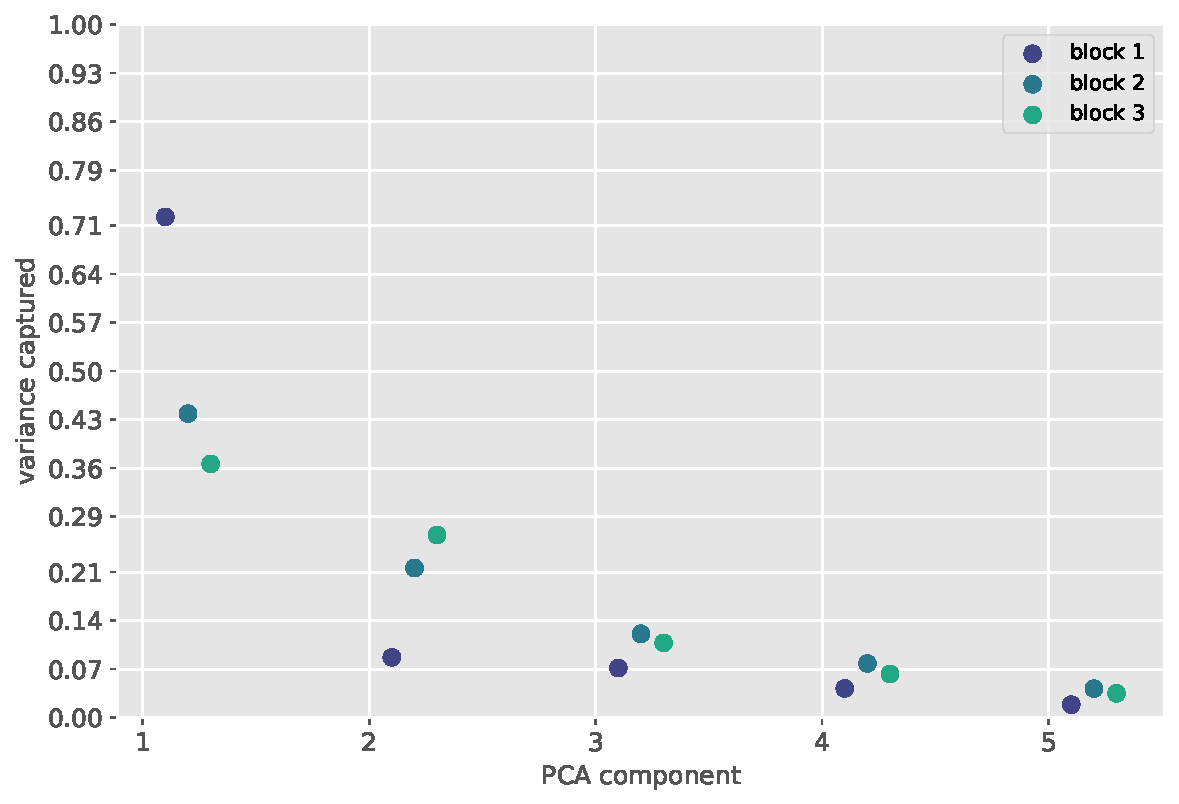
\includegraphics[width=0.2\textwidth]{images/data_analysis/center_hold/PCA_concat_variance.pdf}
% \caption{Fraction of variance captured by PCA computed on concatenated EMG time series concatenated over trials. Over blocks, we see variance shifting from the top component to other components. We hypothesize that across learning we would see the development of bespoke modes used in combination to reach individual targets. This would predict an increase in the complexity of the EMG time series over learning. Here we see suggestions of this prediction.}\label{fig:PCA_concat_variance}
% \end{figure}


% We first asked whether PCA applied to each individual trial would extract a single, high-variance component reflecting the dimensionality of the behavior. Since each finger movement is intuitively one dimensional, we predict that PCA would find a single high-variance component when run on each individual trial. As shown in \Cref{fig:PCA_variances}, this is generally the case, though there are some outlier trials. After inspecting these outlier trials, it is likely that the subject moved multiple fingers in these trials counter to the experimenter's instruction.

% \begin{figure}[H]
% \phantomsection\label{fig:PCA_variances}
% \centering
% 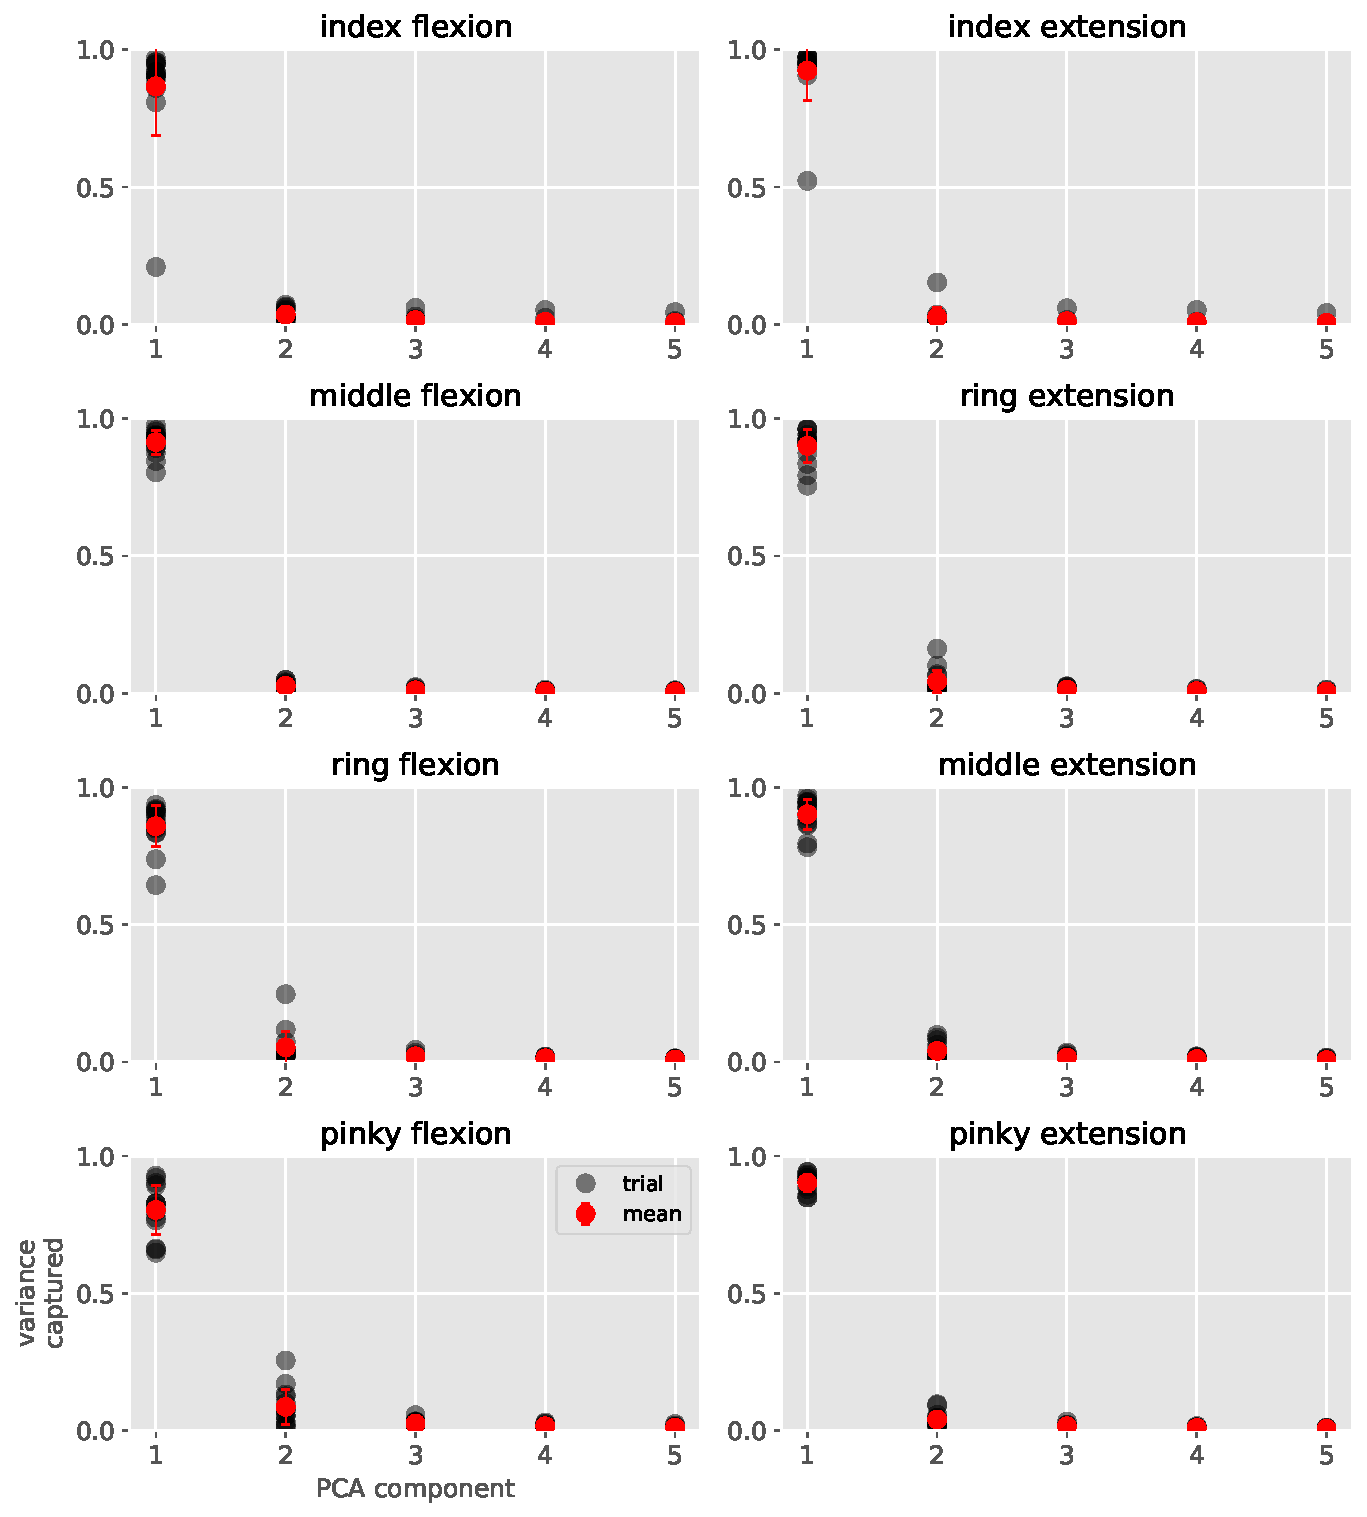
\includegraphics[width=0.2\textwidth]{images/data_analysis/fingers/PCA_variances.pdf}
% \caption{Fraction of variance captured by the top 5 principle components for trials of single finger extensions and flexions. PCs were computed for individual trials. Trials were recorded from one subject for 10s each trial with finger movement frequency approximately 1Hz. Three blocks each with one trial per finger movement were recorded per day for 5 days for a total of 15 trials per finger. Electrodes were not removed between blocks but were removed between days. Each trial displays a single high-variance PC component.}\label{fig:PCA_variances}
% \end{figure}

% We next asked, since each trial appeared to be dominated by a single principle component, whether this top component was stable across trials and across days. If the top component is stable, it implies that the recording apparatus is robust to electrode movement between sessions. The top components for each movement after running PCA on each trial are shown in \Cref{fig:PCA_components}. While it is not typical to run PCA on individual trials, for the purpose of visually inspecting the PCA weights over EMG channels it is used here.

% \begin{figure}[H]
% \phantomsection\label{fig:PCA_components}
% \centering
% 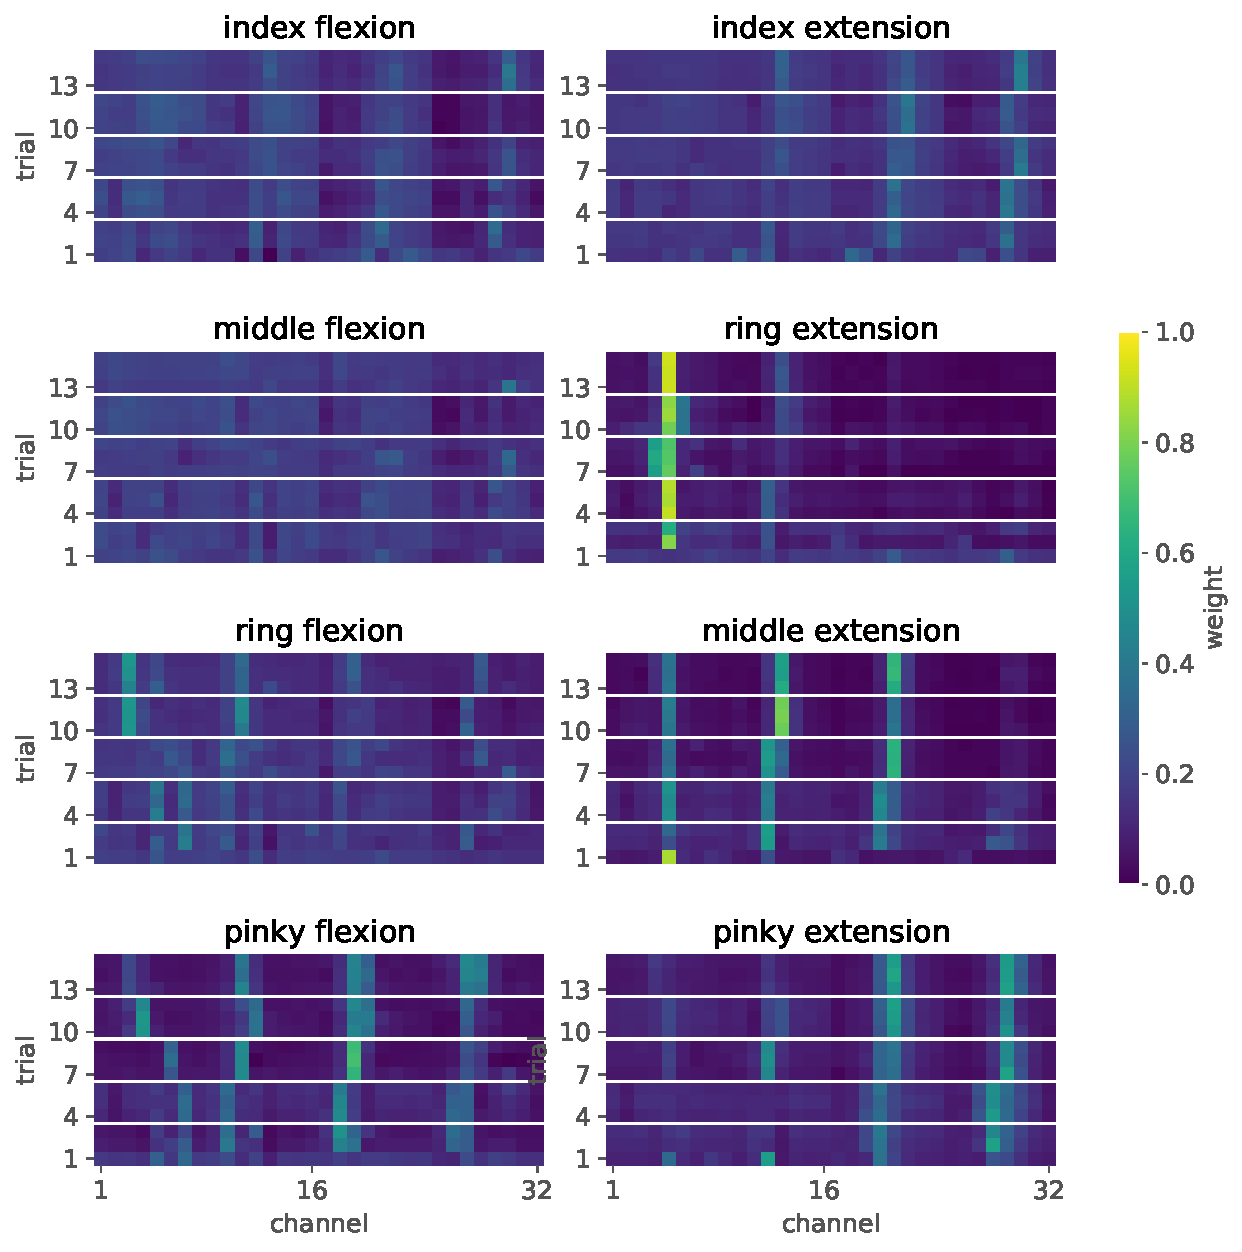
\includegraphics[width=0.2\textwidth]{images/data_analysis/fingers/PCA_components.pdf}
% \caption{The top principle component from each single finger movement trials plotted as weights across channels. PCA was computed for each trial individually. White horizontal lines show breaks between days when electrodes were removed and reapplied. Each trial's top component is relatively stable across trials and across days, though there is drift and dropout of weights. Measures to increase cross-session stability are discussed in the main text. Movements appear to vary between strong localization on single channels and broad activation across channels.}\label{fig:PCA_components}
% \end{figure}

% The results here suggest that, at least up to linear decompositions, the features of low-contraction movements is relatively robust across sessions. As discussed in {section:next\_steps}, we will construct more reliable means to place electrodes on subjects' forearms to further increase repeatability. Another aspect of these results is our assumption subjects are producing the same contraction each time they move their finger, and at the same contraction level. That is, we assume they are recruiting the same motor units each movement. This may not be the case, and constructing new analyses which infer motor unit activations may be useful to mitigate this issue.


% \section[short]{Task Space}

% Visualize trajectories and their statistics nicely
% Visualize trajectories
% Figure out how to compare across targets (rotating?)
% Trends in trajectory stats? Means and variances of histograms



% \begin{figure}[H]
% \centering
% 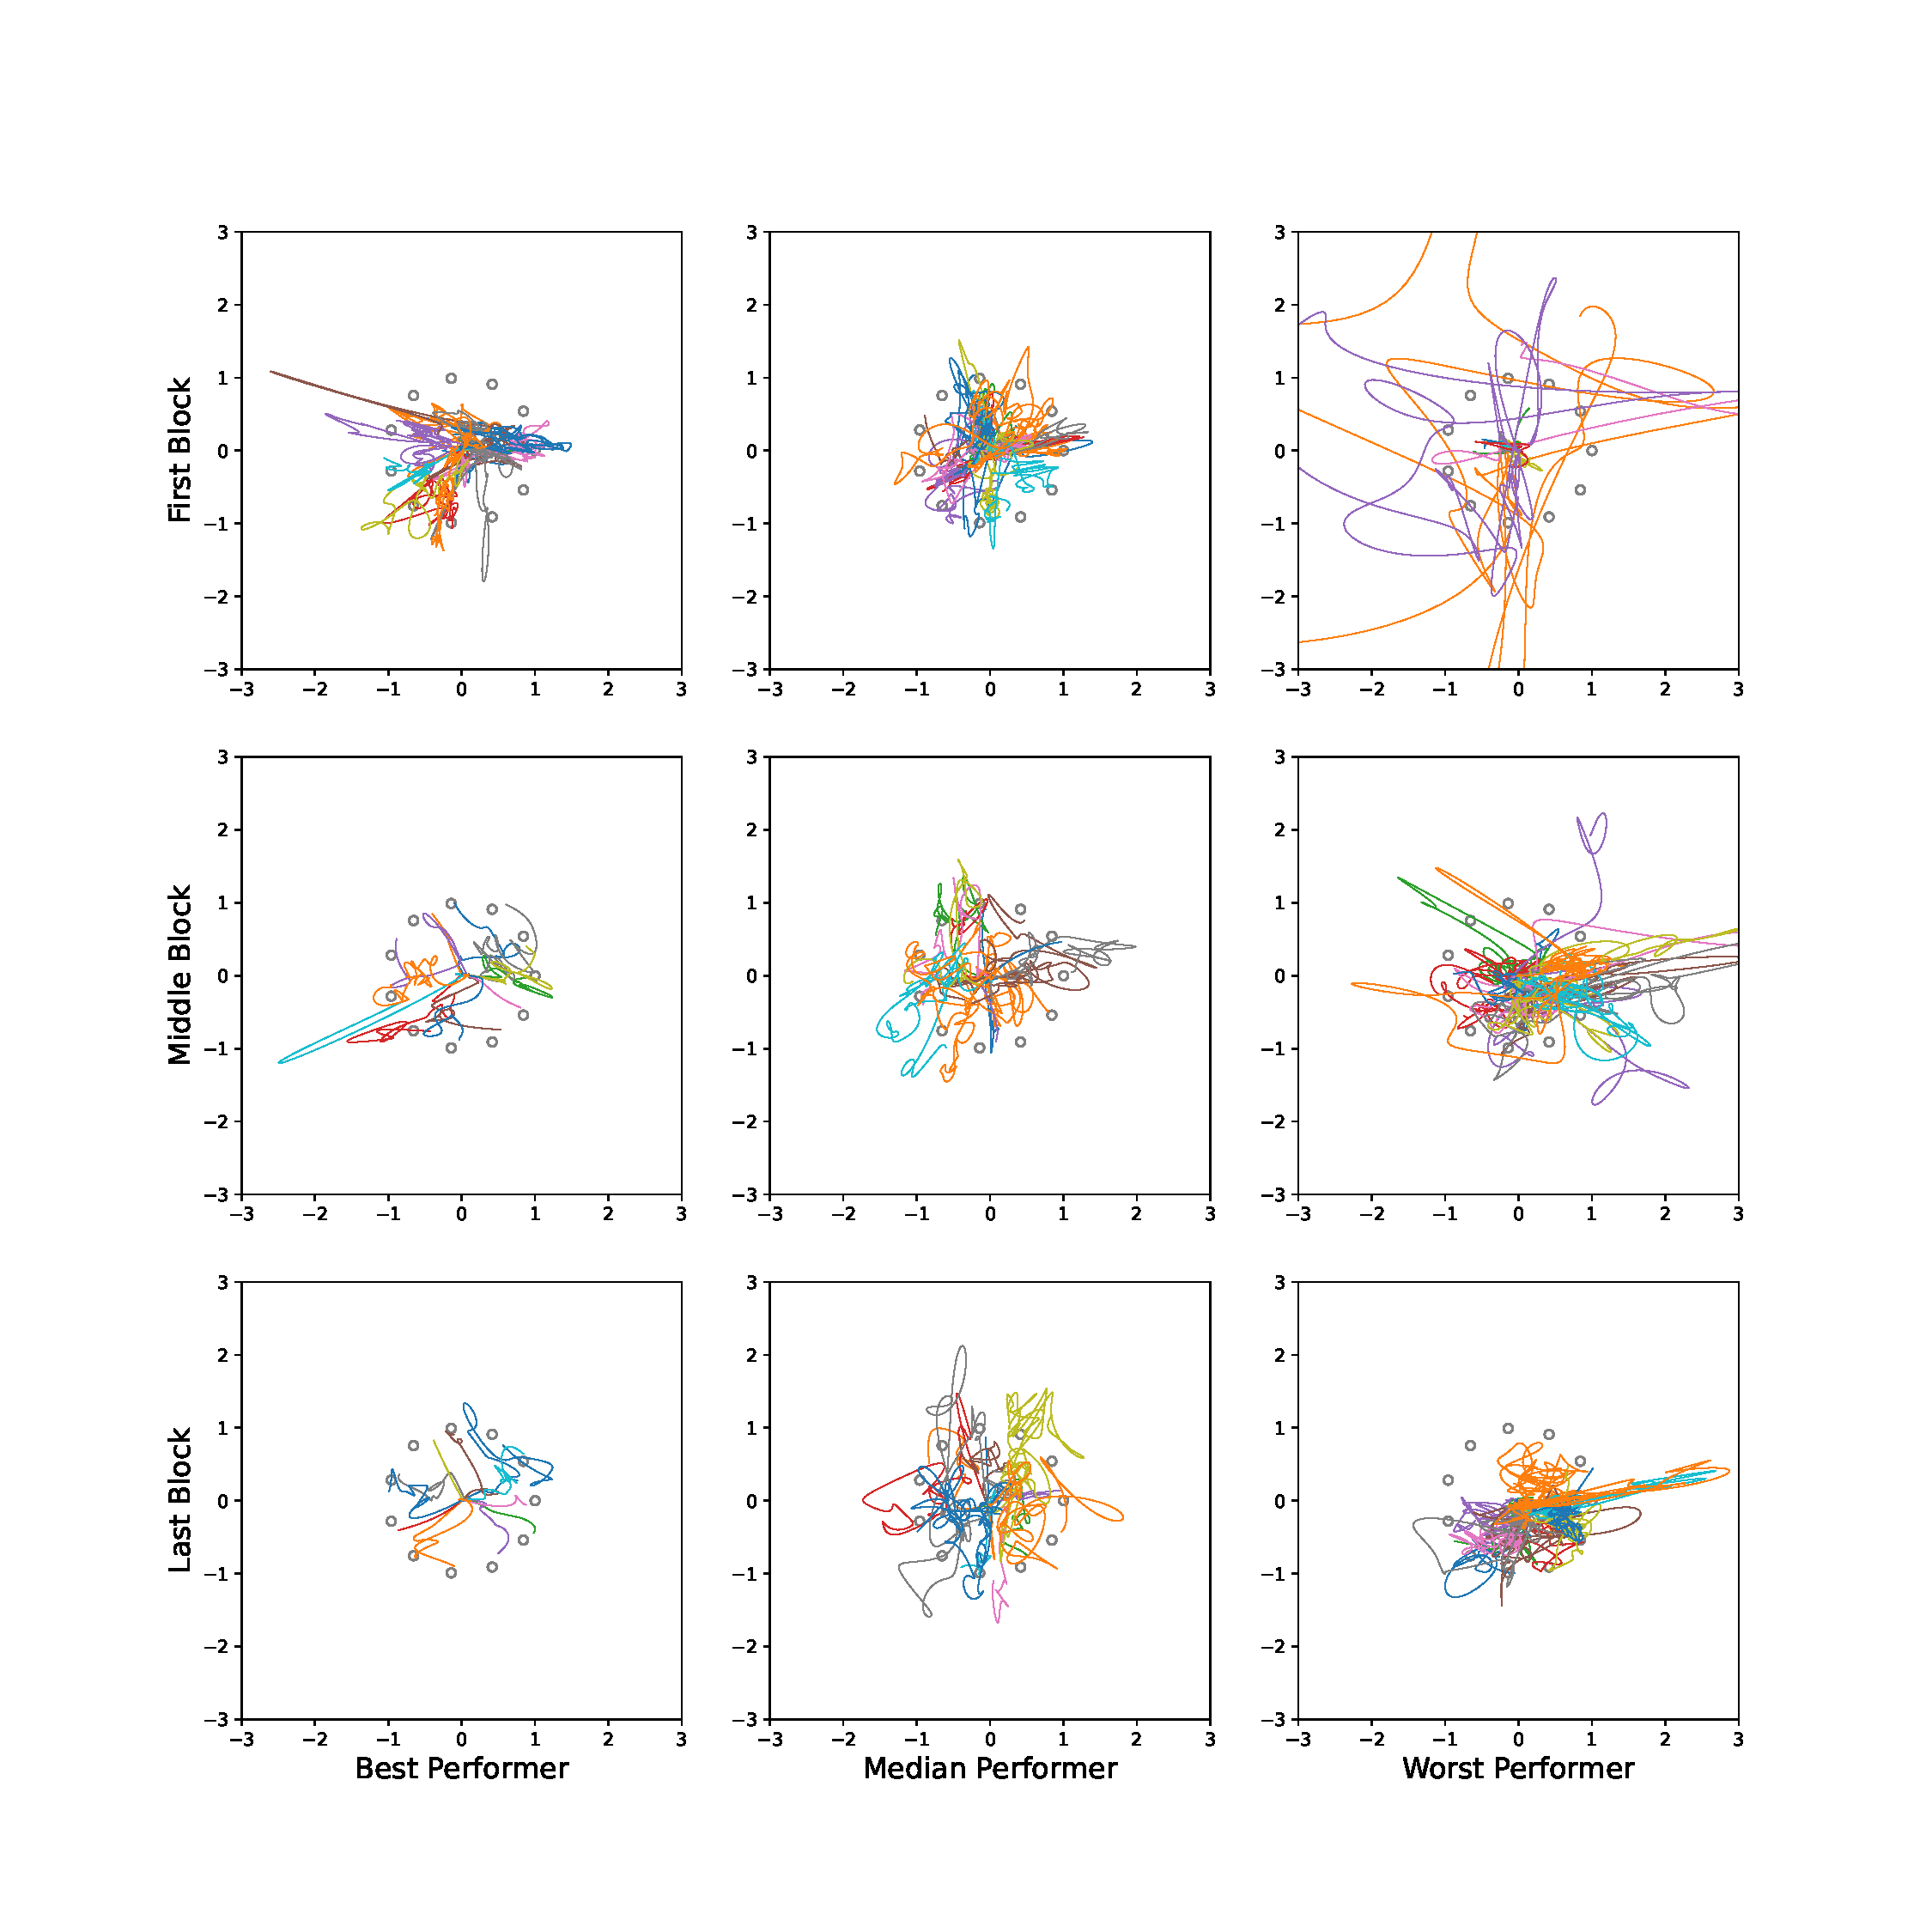
\includegraphics[width=\textwidth]{analysis/behavior.pdf}
% \caption{Example task behavior. Behavioral trajectories from the
% ``center hold, reach out'' task. This task required subject to maintain
% their cursor in the center of the frame by refraining from any muscle
% activity in the recorded forearm for 2s. After this initial period, one
% of 12 targets appeared on-screen (shown here as grey circles). The
% subject attempted to activate their forearm muscle activity to ``reach''    
% to each target. Moving their cursor to the target resulted in a ``Hit''.
% The cursor was allowed to exit the ``screen'' spanning {[}-2,2{]} as
% plotted here, becoming invisible to the subject. Each plot shows cursor
% trajectories from a single block of 12 unique targets, each trial a
% different color. Each column of three plots is a single subject, from
% left to right: the subject with the most, median, and least ``Hits'
% across all trials of the task. Each row shows one block of 12 trials,
% from top to bottom: the first block, the halfway point, and the last
% block.}\label{fig:behavior}
% \end{figure}

% \begin{figure}[H]
% \centering
% 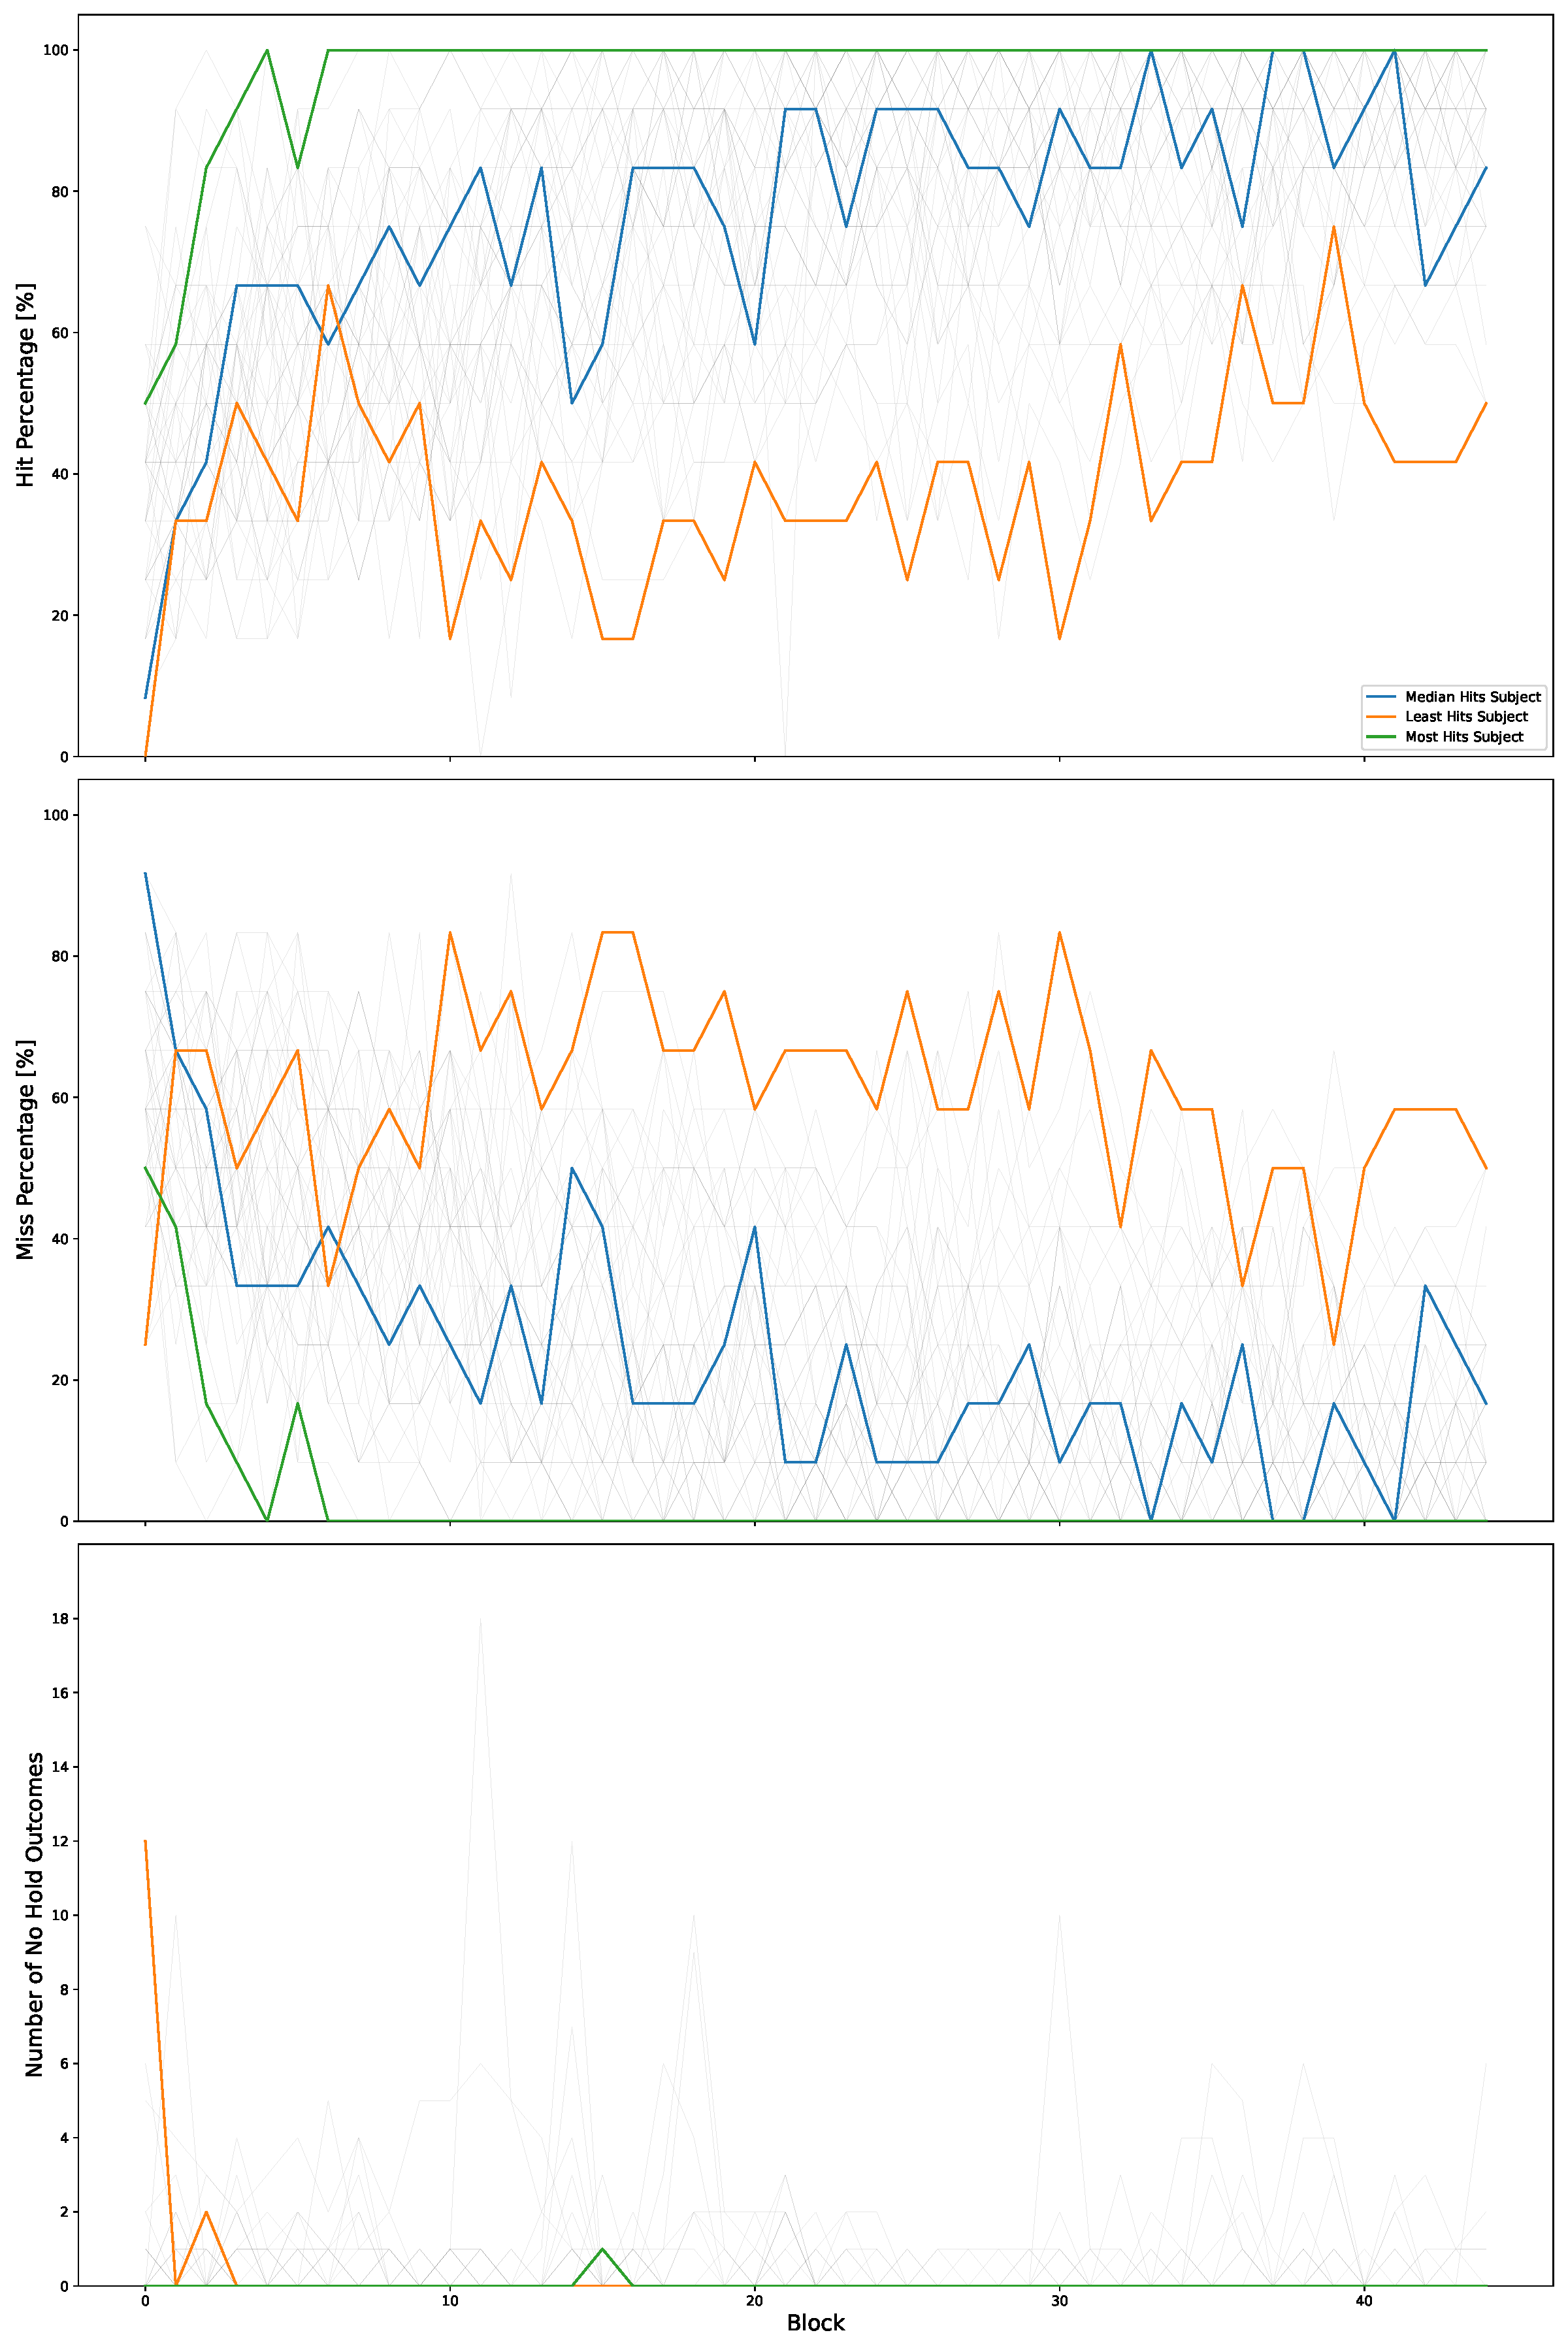
\includegraphics[width=\textwidth]{analysis/outcomes.pdf}
% \caption{Task outcomes over blocks. Outcomes across all 45 blocks of 12
% trials (targets) in the ``center hold, reach out'' task. Subjects with
% the most, median, and least hits are shown in green, blue, and orange
% respectively. All ofther subjects are show in gray. From top to bottom:
% The percentage of ``Hits'' within each block, the percentage of
% ``Misses'' (timeouts), and ``No Holds'' (subject unable to quiet forearm
% muscle activity initially).}\label{fig:outcomes}
% \end{figure}

% \begin{figure}[H]
% \centering
% 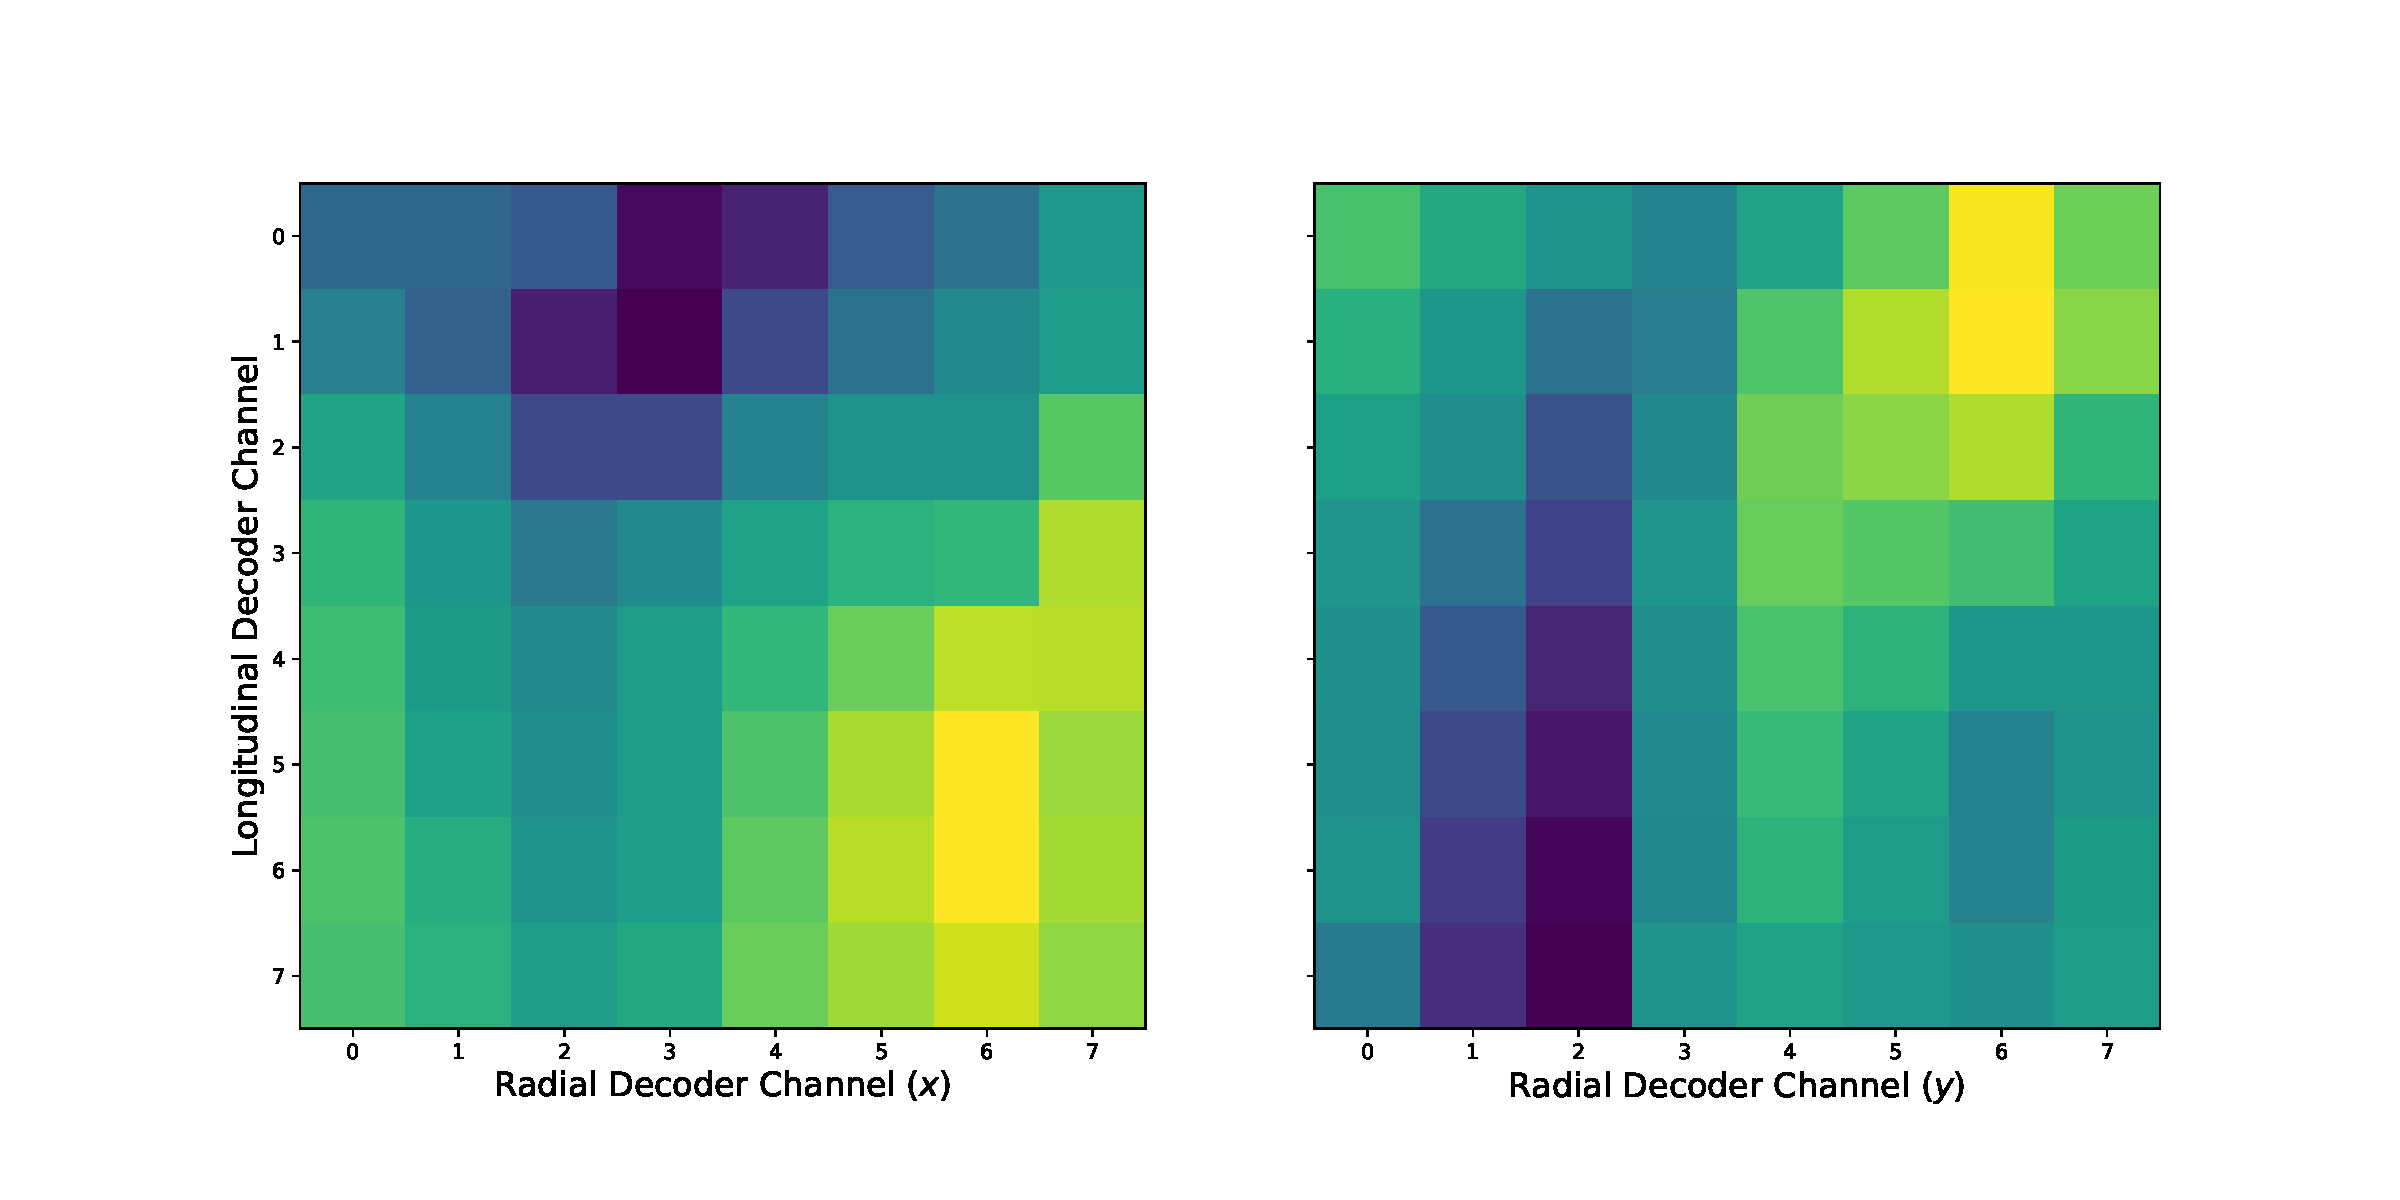
\includegraphics[width=\textwidth]{analysis/decoder_heatmap.pdf}
% \caption{Example EMG-to-force decoders from a single subject. The
% ``center hold, reach out'' task works by mapping 64 channels of EMG
% activity from subjects' forearms to a 2-dimensional force vector, a
% component acting in the \(x\) and \(y\) directions within the task's
% linear dynamics. Depicted here are the two 64-dimensional ``decoders''
% arranged as the EMG electrodes were arranged on subjects' arms (along
% the arm, longitudinally, and around the arm, radially). The left plot
% shows the \(x\) force decoder, and the right plot the
% \(y\).}\label{fig:decoders}
% \end{figure}

% \begin{figure}[H]
% \centering
% 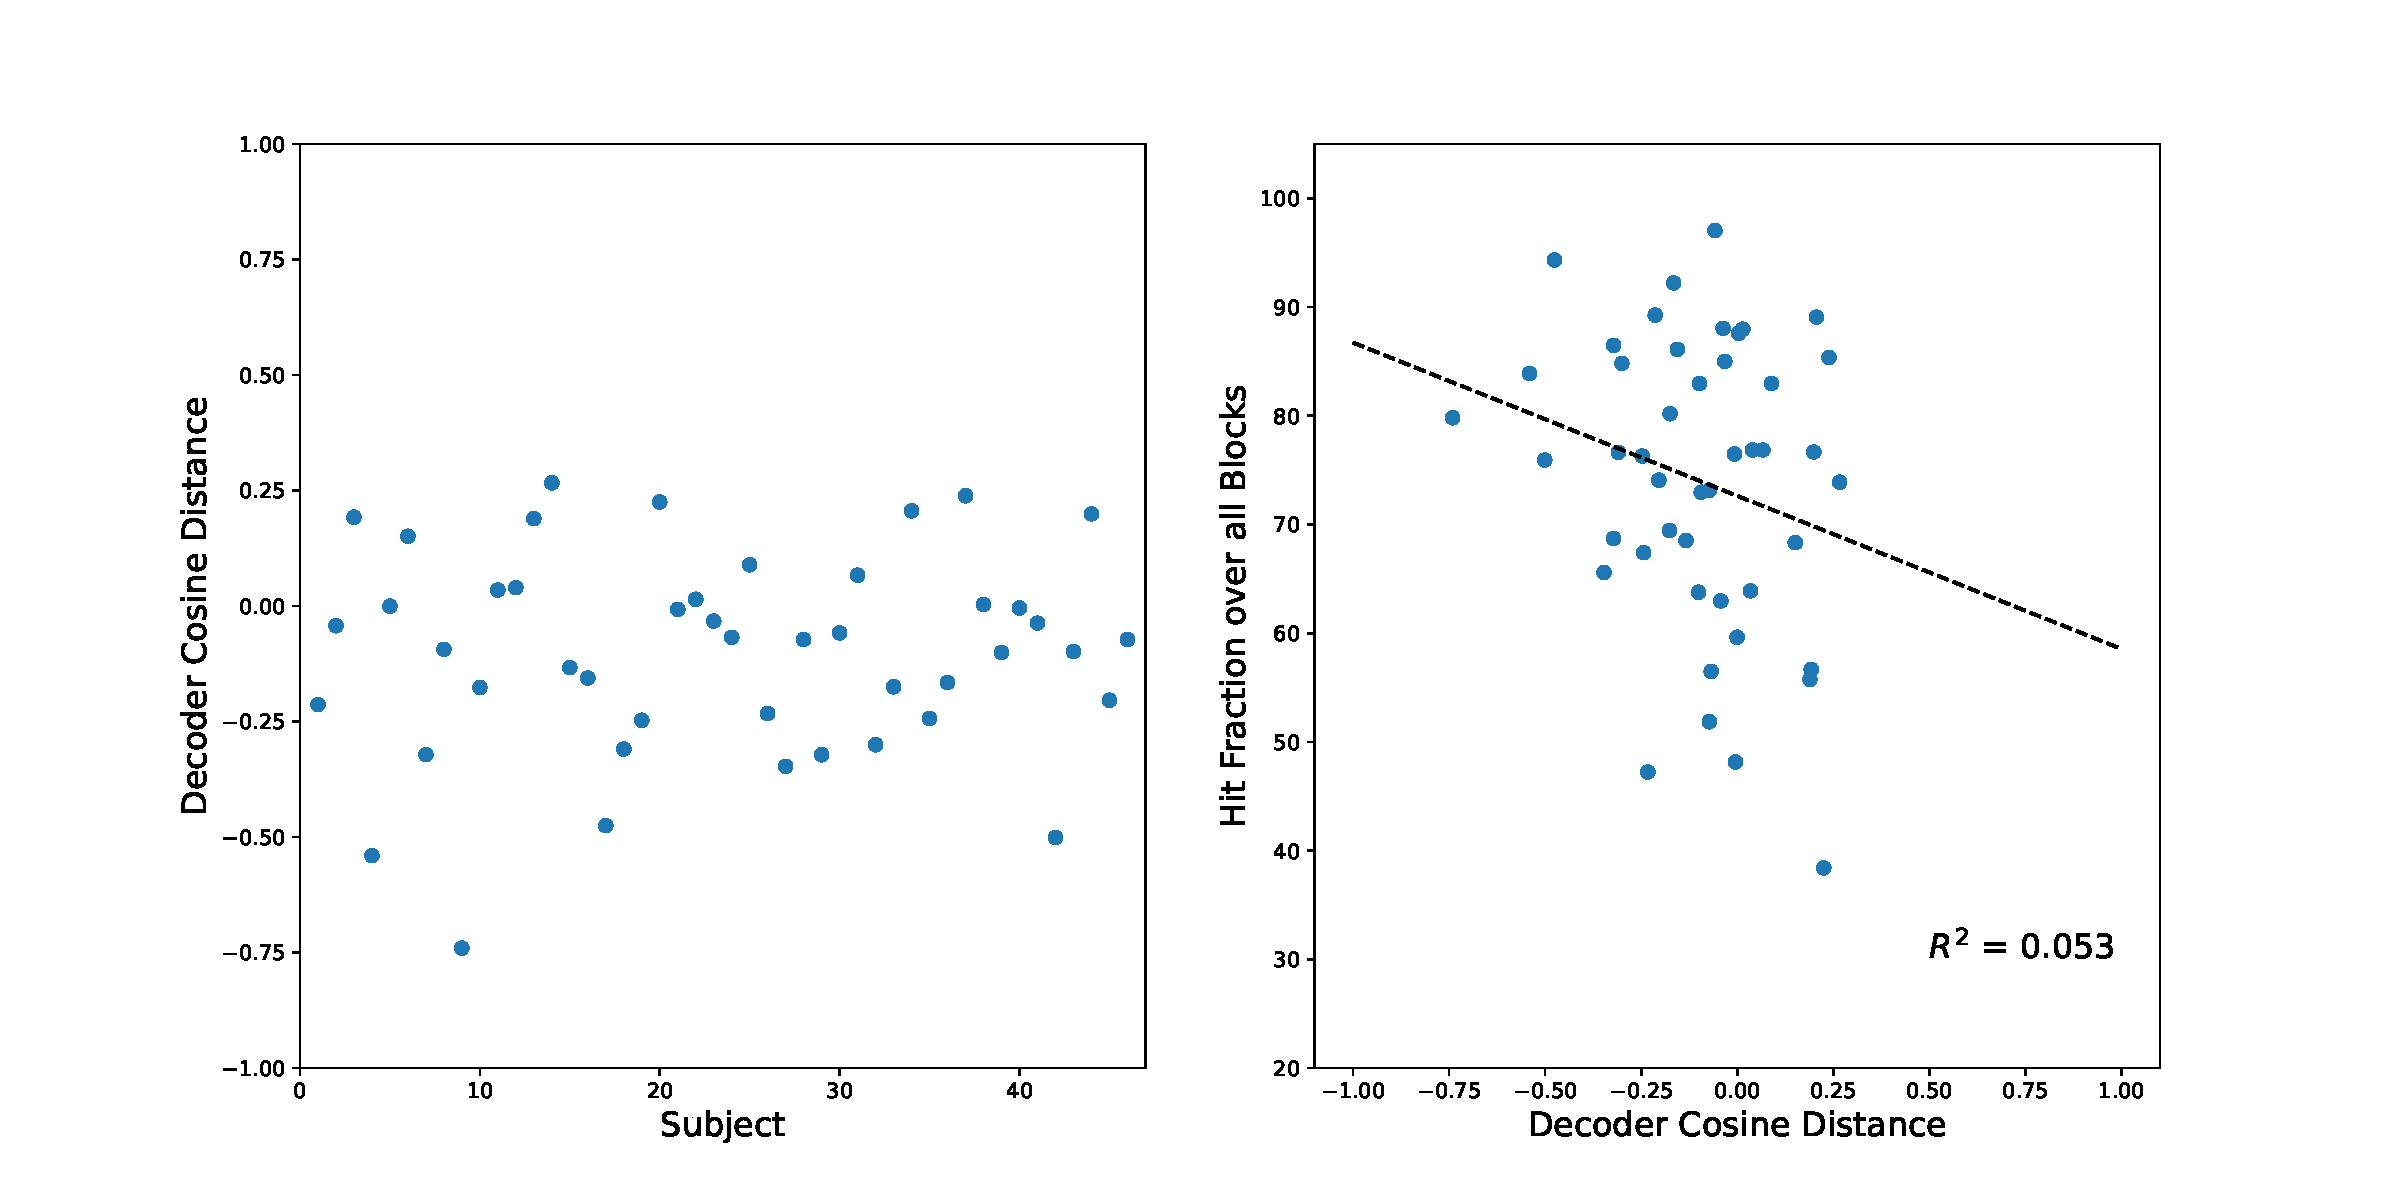
\includegraphics[width=\textwidth]{analysis/decoder_correlation.pdf}
% \caption{Decoder cosine similarity. EMG-to-force decoders are computed
% using a calibration dataset collected before the ``center hold, reach
% out'' task. 4 ``modes'' of EMG activity are extracted from the dataset
% using non-negative matrix factorization. These 4 modes are then
% subtracted in pairs to yield the two 64-dimensional EMG-to-force
% mappings, shown in \{+@fig:low\_variance\_PCs\}. The left plot shows the
% cosine similarity of the \(x\) and \(y\) EMG-to-force decoders. A cosine
% similarity of 1 means the two vectors are parallel, producing identical
% forces (in the respective directions) for the same EMG activity
% (\(F_x = F_y\)). A cosine similarity of -1 means the vectors are
% antiparallel, producing equal but opposite forces in the two directions
% (\(F_x = -F_y\)). A cosine similarity of 0 means the decoder directions
% are orthogonal; e.g.~producing a force in the \(x\) direction with a
% certain EMG activity produces no force in the \(y\) direction. Plotted
% across subjects, we see a range of decoder similarities, providing a
% variety of task contingencies. The rightmost plot asks whether cosine
% similarity is predictive of task success, in terms of the numbers of
% ``Hits''. We find no significant correlation, implying that the decoder
% cosine similarity, in the range we tested, does not predict task
% success. Task success, therefore, likely relies on an alternative task
% variable.}\label{fig:decoder_correlations}
% \end{figure}

% \begin{figure}[H]
% \centering
% 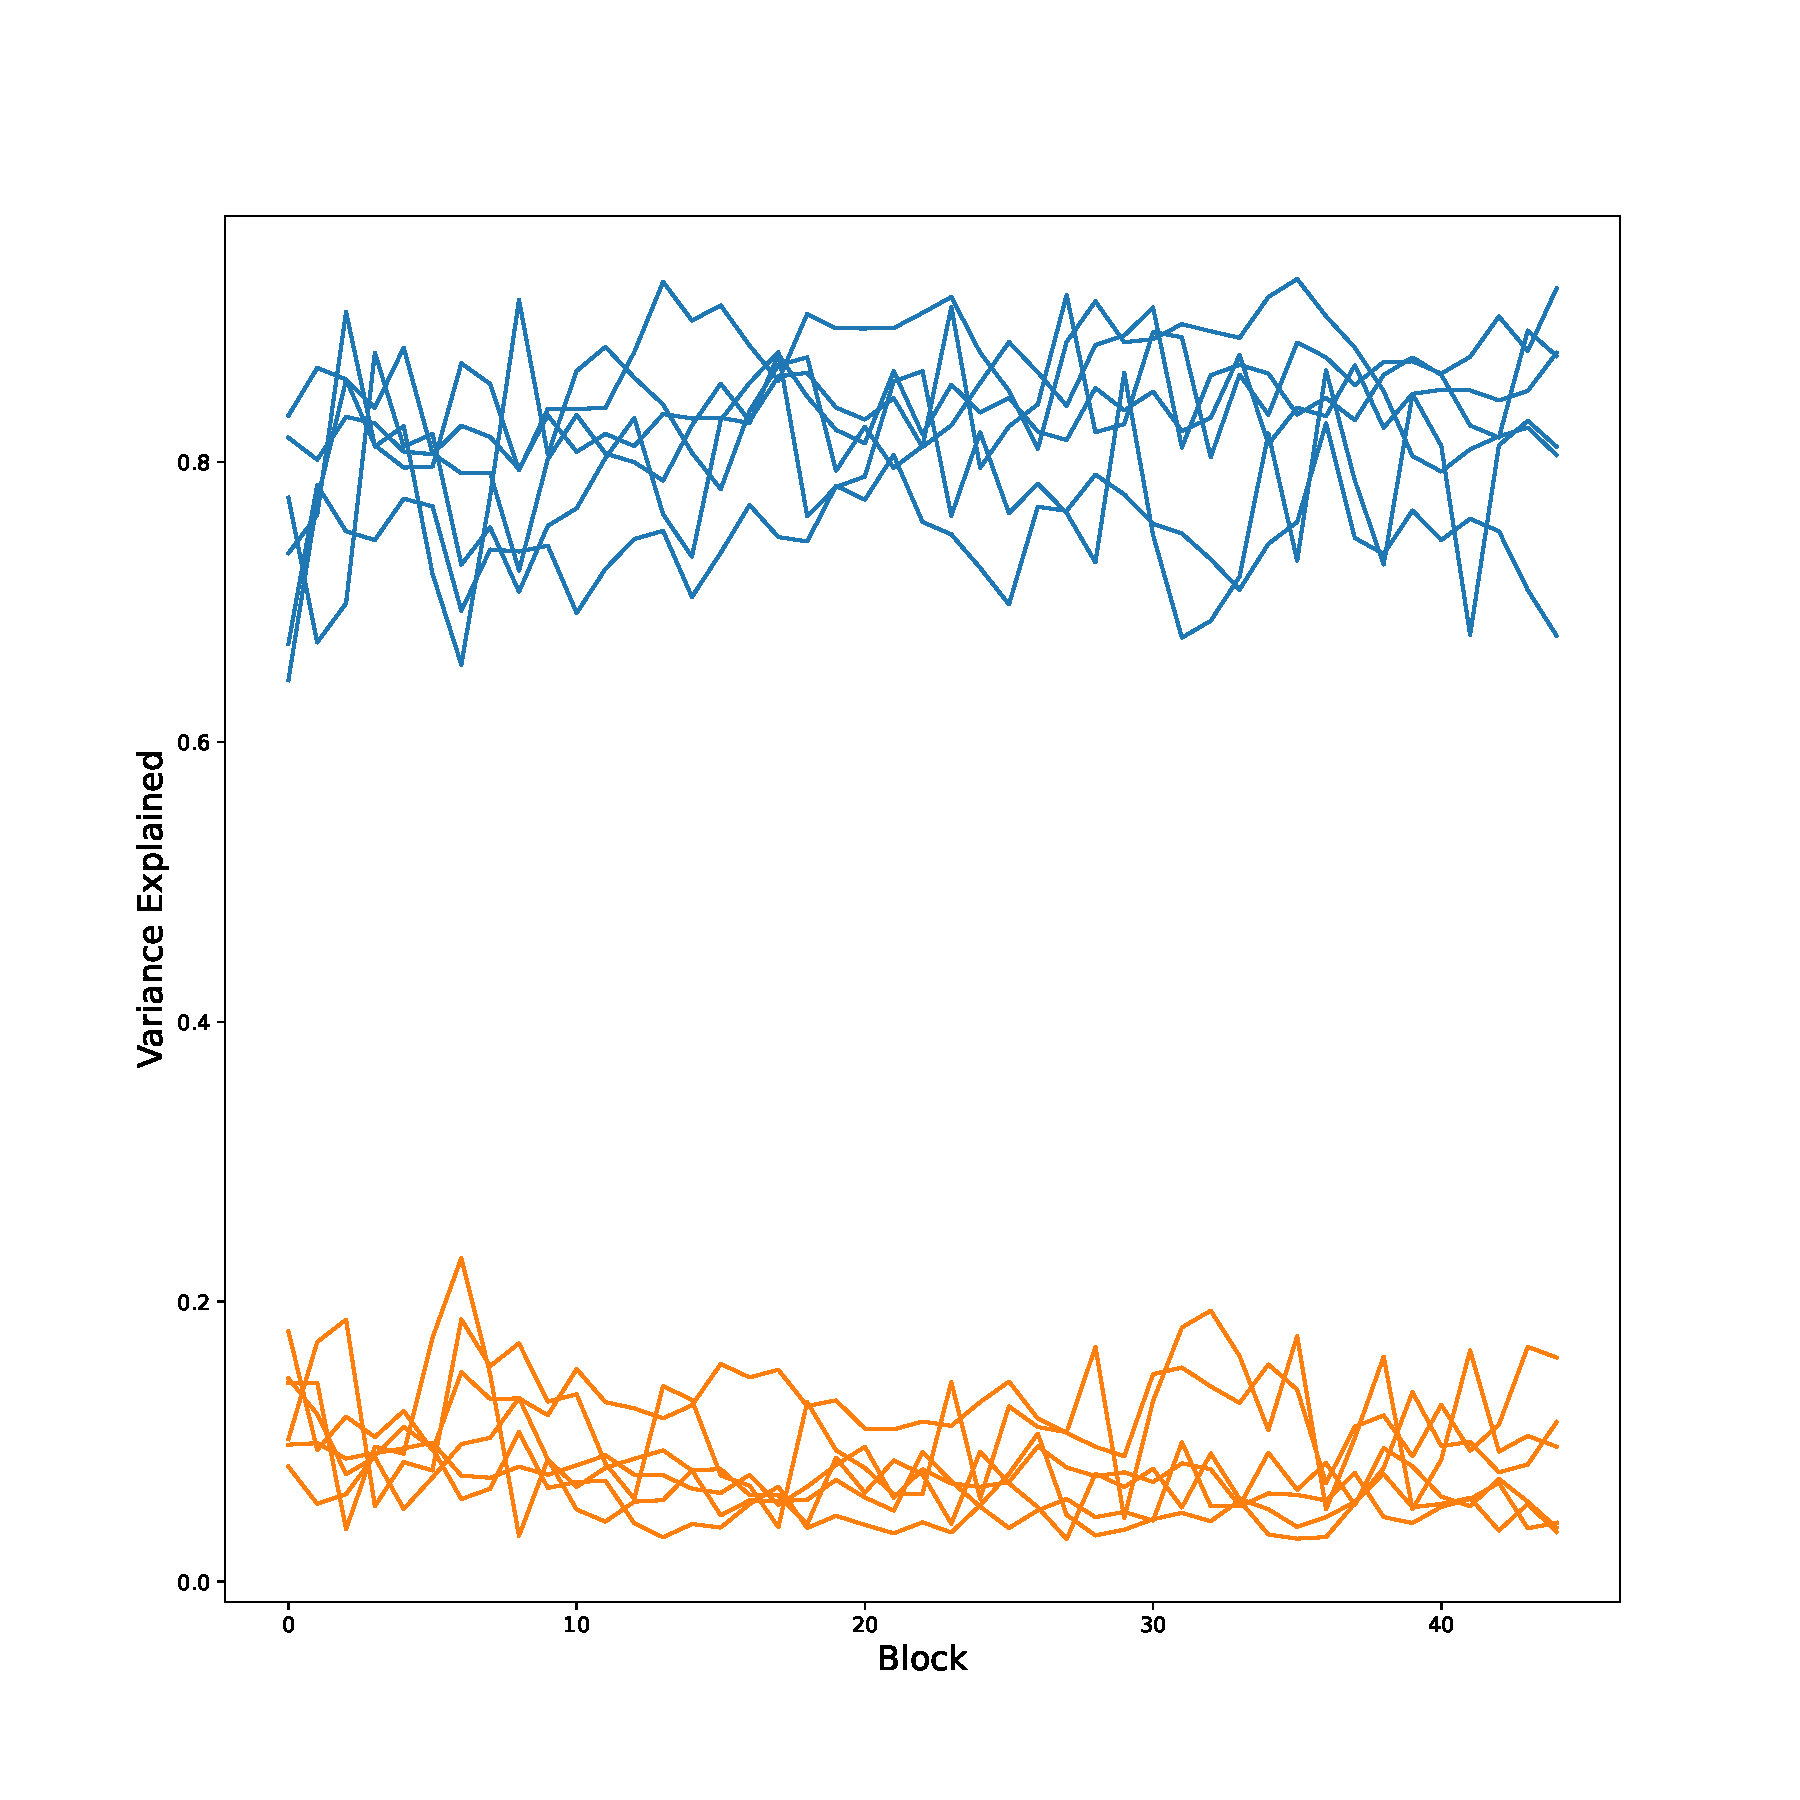
\includegraphics[width=\textwidth]{analysis/PCA_blocks.pdf}
% \caption{PCA of EMG activity over blocks. The experimental paradigm is
% unique in that we have access to the true subject state (EMG activity),
% control over the contingency (the decoding from EMG to force in the
% task), and the outcome (task behavior). This plot addresses the question
% of whether there is a dynamic, over blocks, of the variance of the EMG
% signals concatenate over blocks (12 trials). The plot suggests this is
% not the case, as the first PCA component of EMG activity, for six
% subjects, explains much of the EMG variance for each block, without any
% visual indiciation of a trend. This is a common finding, and confirms
% what is often found in the literature, that joint and/or muscle
% activity, while high-dimensional, displays low dimensional modes.
% Exploring the structure of the variance of this signal is a next step,
% to understand how subjects manage the variability of their activity to
% acheive task success, and how this evolves over
% trials.}\label{fig:behavior}
% \end{figure}


\cleardoublepage\printendnotes%
\ifSubfilesClassLoaded{%
    \newpage%
    \bibliography{../bib/bibliography}%
}{}%
\end{document}